%!TEX root = ../chapter2.tex
%******************************
%	 Results 
%*****************************

\section{Extending the  BASiCS model}

Unlike bulk RNA sequencing, scRNA-Seq provides information about cell-to-cell expression heterogeneity within a population of cells. Past works have used a variety of measures to quantify this heterogeneity. Among others, this includes the coefficient of variation \citep[CV,][]{Brennecke2013} and entropy measures \citep{Richard2016}. The BASiCS model \citep{Vallejos2015BASiCS, Vallejos2016} which was introduced in section \ref{sec0:BASiCS} focuses on biological \textit{over-dispersion} as a proxy for transcriptional heterogeneity. This is defined by the excess of variability that is observed with respect to what would be predicted by Poisson sampling noise, after accounting for technical variation. 

\subsection{The BASiCS model}

As a reminder: Let $X_{ij}$ be a random variable representing the expression count of gene $i$ ($ \in \{1, \ldots, q\}$) in cell $j$ ($\in \{ 1, \ldots ,n\}$).  To control for technical noise, we employ reads from synthetic RNA spike-ins (see \citep{Jiang2011}). We assume the first $q_0$ genes to be biological followed by the $q-q_0$ spike-in genes. BASiCS assumes a hierarchical Poisson formulation: 

\begin{equation} \label{eq::PoissonBASiCS}
 X_{ij}|\mu_i,\phi_j,\nu_j,\rho_{ij} \ind
 \left\lbrace
  \begin{aligned}
    &\text{Poisson}(\phi_j\nu_j\mu_i\rho_{ij}), && i=1,...,q_0,j=1,...n;  \\ 
    &\text{Poisson}(\nu_j\mu_i), && i=q_0+1,...,q,j=1,...,n,    	    
  \end{aligned}
\right.
\end{equation} 

where, to account for technical ($\nu_j$) and biological ($\rho_ij$) factors that affect the variance of the transcript counts, we incorporate two random effects: 

\begin{equation} \label{eq::RandomEffectsBASiCS}
\nu_j|s_j,\theta \ind \text{Gamma}\left(\frac{1}{\theta},\frac{1}{s_j\theta}\right), \hspace{0.5cm} \rho_{ij}|\delta_i  \ind \text{Gamma}\left(\frac{1}{\delta_i},\frac{1}{\delta_i}\right)\\
\end{equation} 

Here, $\phi_j$ represents a cell-specific normalization parameter to correct for differences in mRNA content between cells and $s_j$ models cell-specific scale differences affecting all biological and technical genes. The strength of the technical noise $\nu_j$ noise is quantified by a global parameter $\theta$ (shared across all genes and cells). The strength of heterogeneous gene expression across cells $\rho_{ij}$ is controlled by gene-specific over-dispersion parameters $\delta_i$ which we used as a proxy for biological expression variability in chapter 1.  Finally, gene-specific parameters $\mu_i$ represent average expression of a gene across cells. \\

As shown in chapter 1, over-dispersion as a measure of variability can be used to identify genes whose transcriptional heterogeneity differs between groups of cells (defined by experimental conditions or cell types). However, the strong relationship that is typically observed between variability and mean estimates (see \textbf{Section \ref{sec0:BASiCS}} and \citep{Brennecke2013}) can hinder the interpretation of these results. 

\newpage

\subsection{Approaches to correct the mean-variability confounding effect}

A simple solution to avoid this confounding was used in chapter 1 by restricting the assessment of differential variability to genes with equal mean expression across populations \textbf{(Fig.~\ref{fig2:Schematic_model}A and Section \ref{sec1:BASiCS})}. However, this is sub-optimal, particularly in the case of naive and activated CD4\plus{} T cells where large sets of genes are differnetially regulated upon immune activation. With the current model, immune response genes (e.g.~cytokines, nuclear receptors, transcription factors) are excluded from differential variability testing. An alternative approach is to directly adjust variability measures to remove this confounding. For example, \cite{Kolodziejczyk2015cell} computed the empirical distance between the squared CV to a rolling median along expression levels --- referred to as the DM method.  \\

In line with this idea, our method extends the statistical model implemented in BASiCS \citep{Vallejos2015BASiCS, Vallejos2016} to meaningfully assess changes in transcriptional heterogeneity when genes exhibit shifts in mean expression \textbf{(Fig.~\ref{fig2:Schematic_model}B)}. For this, we infer a regression trend between over-dispersion ($\delta_i$) and gene-specific mean parameters ($\mu_i$), by introducing a joint informative prior to capture the dependence between these parameters. A latent gene-specific \textit{residual over-dispersion} parameter $\epsilon_i$ describes departures from this trend \textbf{(Fig~\ref{fig2:Schematic_model}C)}. The value of $\epsilon_i$ indicates whether a gene exhibits more (positive) or less (negative) variation than expected relative to genes with similar expression levels. Importantly, this measure is not confounded by mean expression \textbf{Fig.~\ref{fig2:Schematic_model}D}. \\

The hierarchical Bayes approach infers full posterior distributions for the gene-specific latent residual over-dispersion parameters $\epsilon_i$. As a result, we can directly use a probabilistic approach to identify genes with large absolute differences in residual over-dispersion between two groups of cells. When the posterior samples of $\epsilon_i$ in condition A are very different from posterior samples of $\epsilon_i$ in condition B, the majority of values for $|\epsilon_i^A - \epsilon_i^B|$ are larger than a given threshold $\psi_0>0$. In this case, the gene is found to be differentially variable between the two conditions  \textbf{(Fig.~\ref{fig2:Schematic_model}E and Section \label{sec0:decision})}. In contrast, mean-corrected point estimates for residual noise parameters (such as those obtained by the DM method) cannot be directly used to perform gene-specific statistical testing between two conditions as no measure of the uncertainty in the estimate is readily available.\\

\newpage

\begin{figure}[!h]
\centering
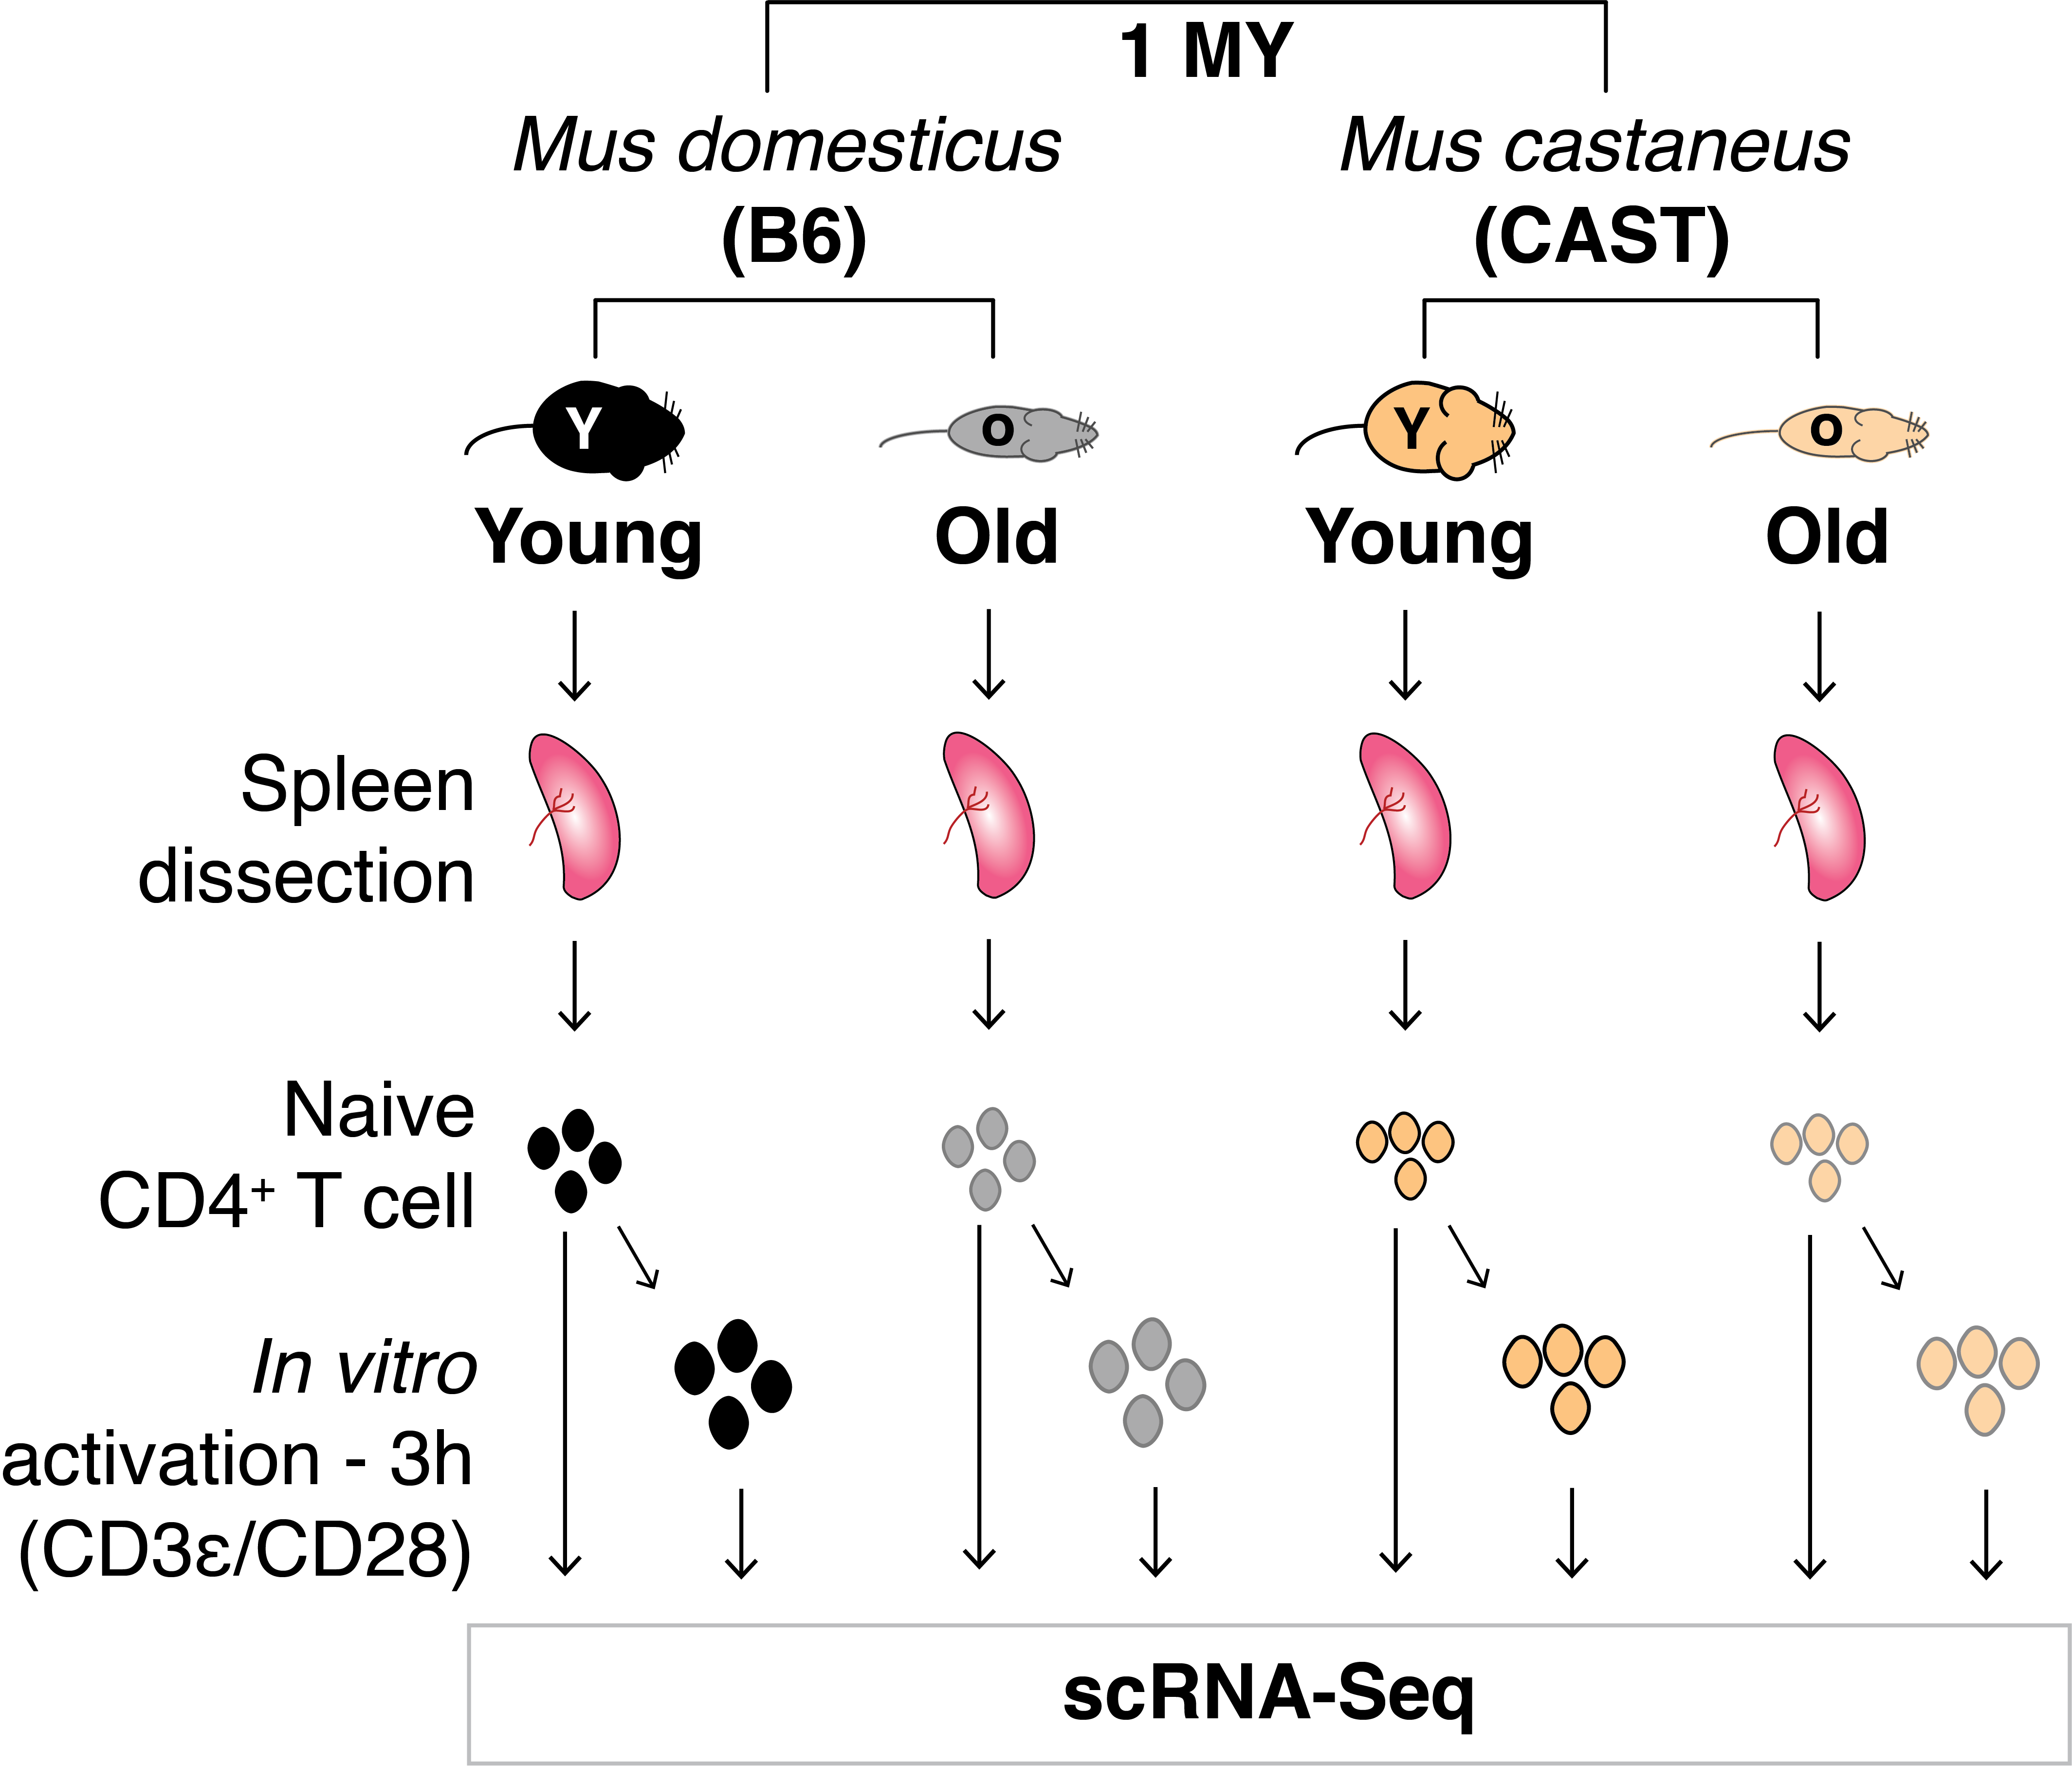
\includegraphics[width=0.9\textwidth]{Fig_1.png}
\caption[Addressing the mean confounding effect in scRNA-Seq data]{\textbf{Addressing the mean confounding effect in scRNA-Seq data (full legend on next page).}\\}
\label{fig2:Schematic_model}
\end{figure}

\newpage

\captionsetup[figure]{list=no}
\addtocounter{figure}{-1}   
\captionof{figure}{\textbf{Addressing the mean confounding effect in scRNA-Seq data (continued).}\\
\textbf{(A and B)} Illustration of changes in expression variability for a single gene between two cell populations without (left) and with (right) changes in mean expression, \textbf{(C and D)} The extended BASiCS model infers a regression trend between gene-specific estimates of over-dispersion parameters $\delta_i$ and mean expression $\mu_i$. Residual over-dispersion parameters $\epsilon_i$ are defined by departures from the regression trend (red arrow). The colour code within the scatterplots is used to represent areas with high (yellow/red) and low (blue) concentration of genes. For illustration purposes, the data introduced by \cite{Antolovic2017} has been used, \textbf{(C)} Illustration of the typical confounding effect that is observed between gene-specific estimates of over-dispersion parameters $\delta_i$ and mean expression parameters $\mu_i$. Genes that are not detected in at least 2 cells are indicated by purple points, \textbf{(D)} Gene-specific estimates of residual over-dispersion parameters $\epsilon_i$ are independent of mean expression parameters $\mu_i$, \textbf{(E)} Illustration of how posterior uncertainty is used to highlight changes in residual over-dispersion. Two example genes with (upper panels) and without (lower panels) changes in residual over-dispersion are shown. Left panels illustrate the posterior density associated to residual over-dispersion parameters $\epsilon_i$ for a gene in two groups of cells (group A: light blue, group B: dark blue). The coloured area in the right panels represents the posterior probability of observing an absolute difference $|\epsilon^A_{i} - \epsilon^B_{i}|$ that is larger than the minimum tolerance threshold $\psi_0$.\\}
\captionsetup[figure]{list=yes}

\subsection{Modelling the confounding between mean and over-dispersion} \label{sec2:extended_BASiCS}

Here, we extend BASiCS to account for the confounding effect described above. In a Bayesian framework, the prior information captures the relationship between parameters. Therefore, we introduce the following joint prior distribution for $(\mu_i, \delta_i)'$: 

\begin{equation} \label{eq::jointprior} \mu_i \sim \text{log-Normal}\left(0, s^2_{\mu}\right), \hspace{0.8cm}
\delta_i | \mu_i \sim \text{log-}\text{T}_{\eta}\left( \text{f}(\mu_i), \sigma^2 \right).
\end{equation} 

The latter is equivalent to the following non-linear regression model:

\begin{equation} \label{eq::regression}
\log(\delta_i) =\text{f}(\mu_i)+\epsilon_i, \hspace{0.5cm} \epsilon_i \sim{}\text{T}_{\eta}(0,\sigma^2), 
\end{equation} where $\text{f}(\mu_i)$ represents the over-dispersion (on the log-scale) that is predicted by the global trend (across all genes) for a given mean expression $\mu_i$. Therefore, $\epsilon_i$ can be interpreted as a latent gene-specific \textit{residual over-dispersion} parameter, capturing departures from the overall trend. \\

A similar approach was introduced by DESeq2 \citep{Love2014} in the context of bulk RNA sequencing. Whereas DESeq2 assumes normally distributed errors when estimating this trend, here we use Student-T distributed errors as it leads to inference that is more robust to the presence of outlier genes. 

\newpage

Moreover, the parametric trend assumed by DESeq2 is replaced by a more flexible semi-parametric approach. This is defined by

\begin{equation} \label{eq::trend}
\text{f}(\mu_i) = \alpha_0 + \log(\mu_i)\alpha_1 + \sum_{l=1}^L \text{g}_l(\log(\mu_i))\beta_l,
\end{equation} 

which is a linear combination of an intercept, a linear term $\log{\mu_i}$ and a set of $L$ Gaussian radial basis function (GRBF) kernels $\text{g}_1(\cdot), \ldots, \text{g}_L(\cdot)$. As in \cite{Kapourani2016}, these are defined as: 

\begin{equation} \label{eq::GRBF}
\text{g}_l(\log(\mu_i)) = \exp\left\lbrace-\frac{1}{2}\left(\dfrac{\log(\mu_i)-m_l}{h_l}\right)^2\right\rbrace, \hspace{0.3cm} l = 1, \ldots, L,
\end{equation} 

where $m_l$ and $h_l$ represent location and scale hyper-parameters for GRBF kernels and $\alpha_0, \alpha_1, \beta_1, \ldots, \beta_L$ are regression coefficients. \\

In \eqref{eq::trend}, the linear term captures the (typically negative) global correlation between $\delta_i$ and $\mu_i$. Its addition also stabilises inference of GRBFs around mean expression values where only a handful of genes are observed. In \eqref{eq::GRBF}, the location and scale hyper-parameters $(m_l, h_l)$ are assumed to be fixed \emph{a priori}. A schematic representation of this regression approach can be seen in \textbf{Fig. \ref{fig2:GRBFs}}.

\begin{figure}[!h]
\centering
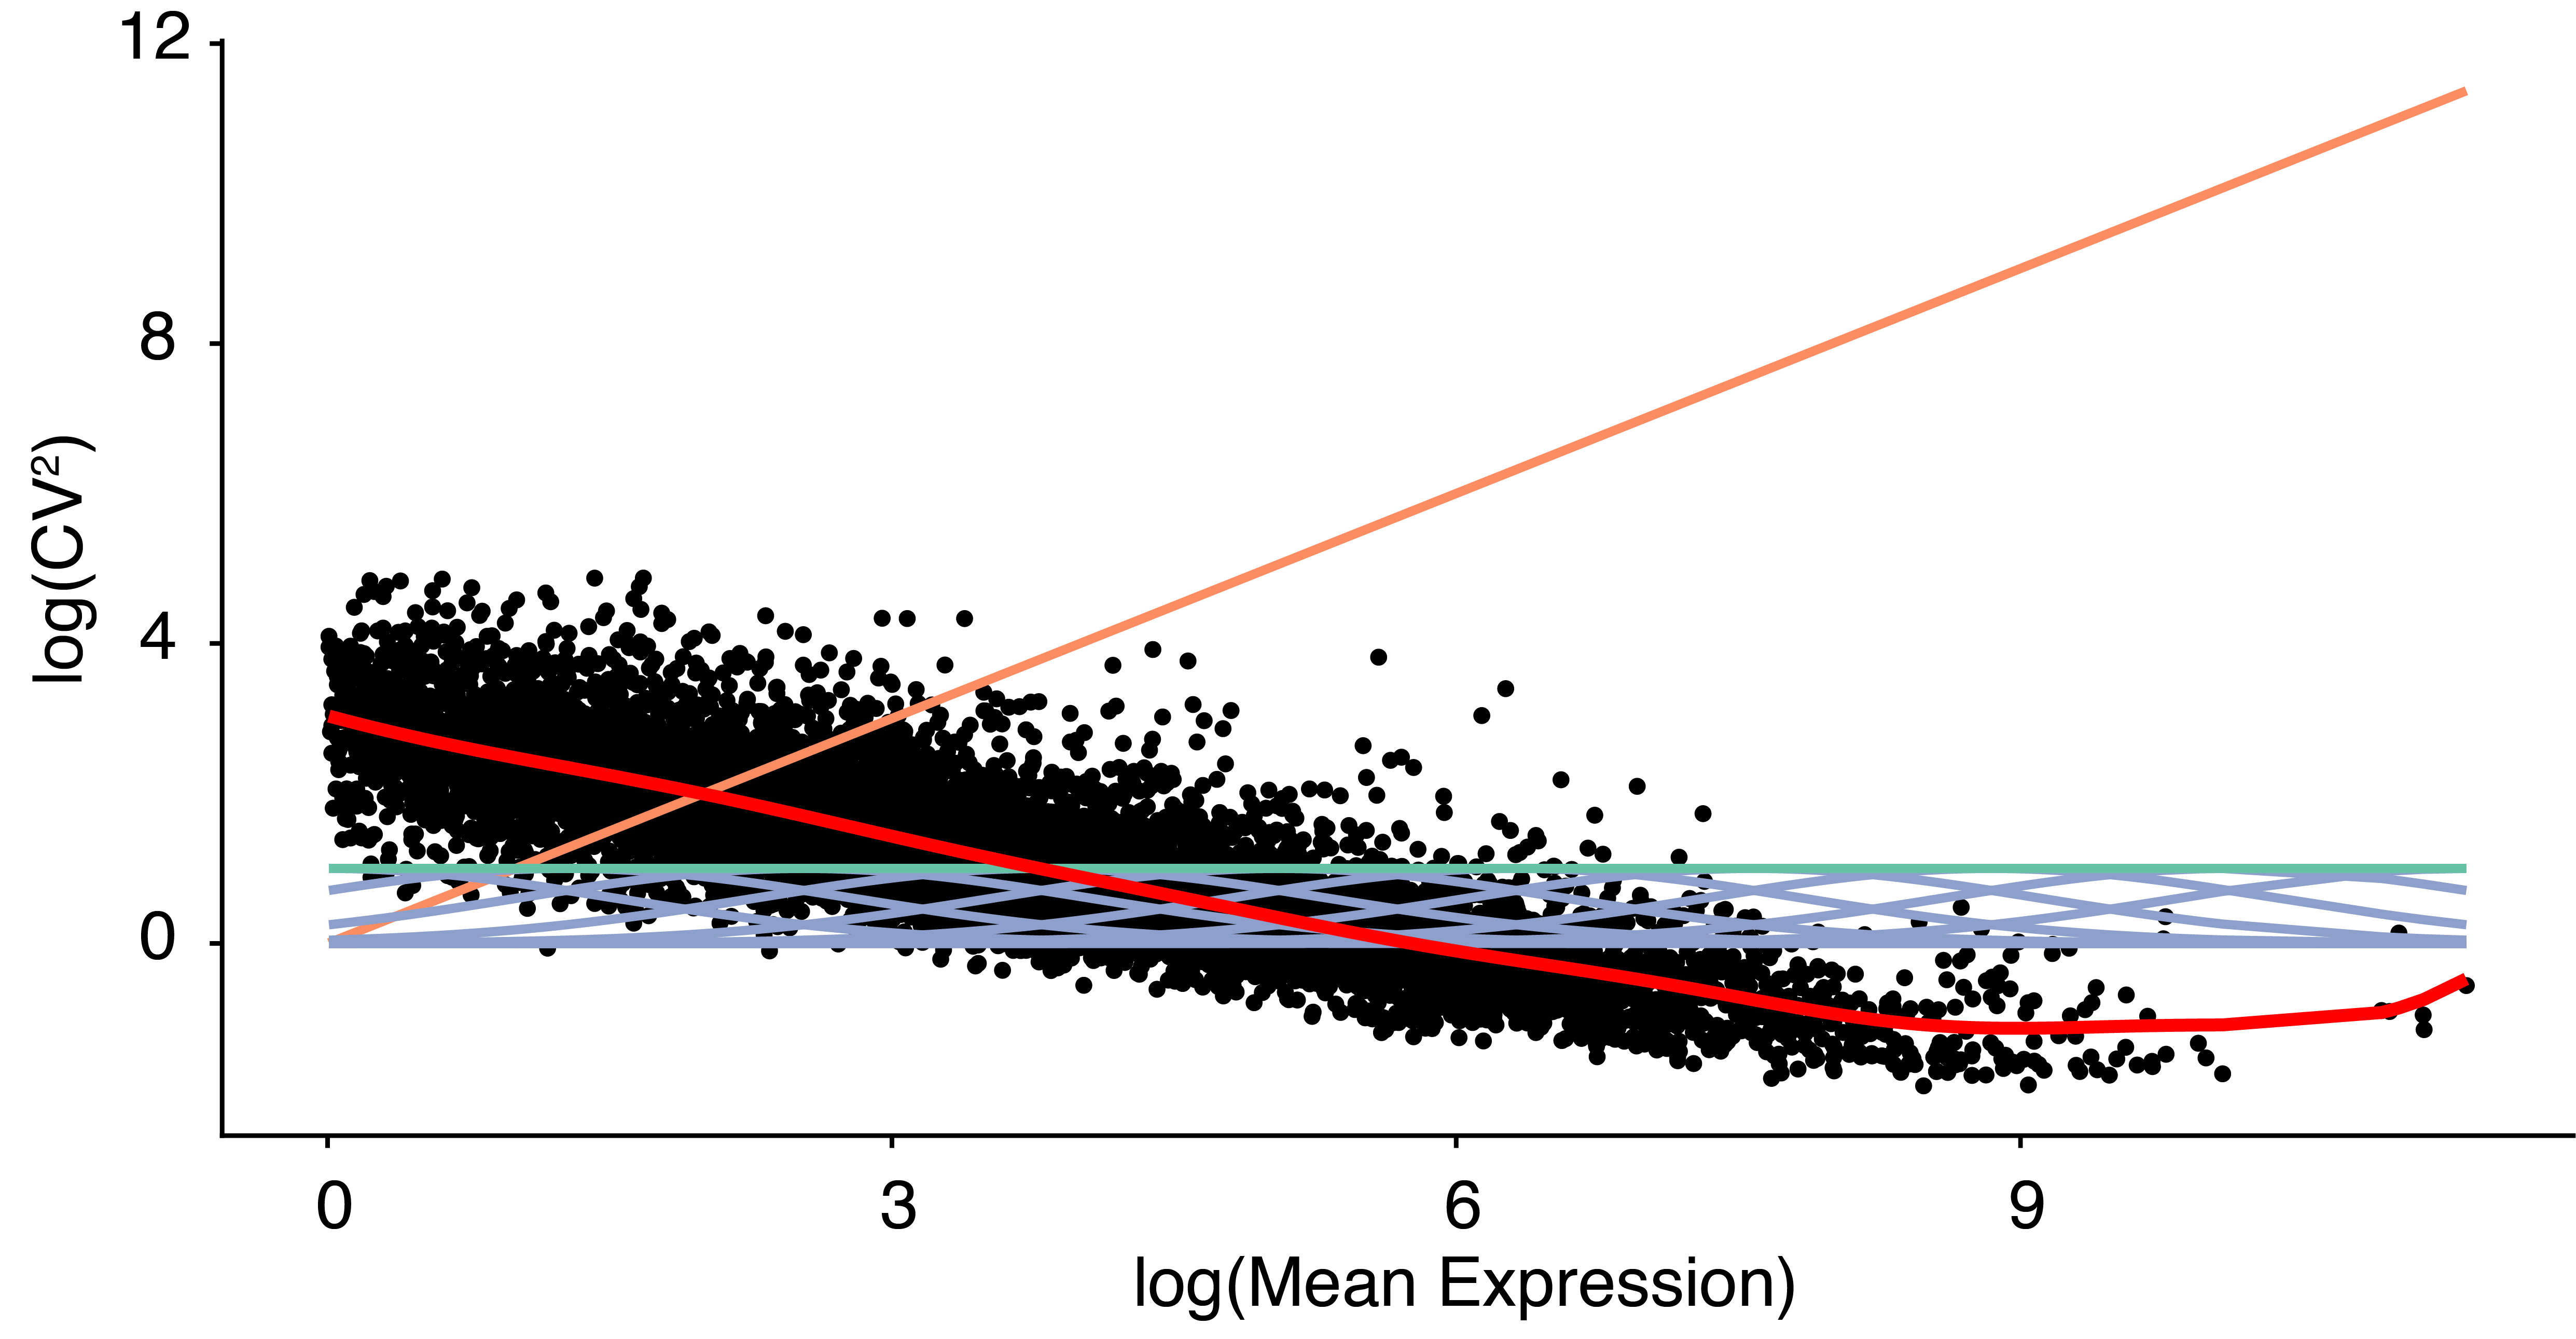
\includegraphics[width=0.9\textwidth]{Fig_2.png}
\caption[Schematic representation of the regression approach using GRBFs]{\textbf{Schematic representation of the regression approach using GRBFs.}\\
Point estimates of the squared coefficient of variation (CV$^2$) were plotted against mean expression. For fitting a regression trend, the model matrix $X$ contains an intercept term (green line), a linear component (orange line) and 10 GRBFs (blue lines). For visualization purposes, a linear regression was fitted using least-square estimates (red line) based on the given model matrix $X$ and data from Dictyostelium at day 0 \citep{Antolovic2017}.}
\label{fig2:GRBFs}
\end{figure}


\subsection{Implementation}

Next, we will give a detailed explanation on how the model was build and how posterior sampling was performed.  


\subsubsection{Prior specification}

For implementation purposes, the log-Student-T distribution in \ref{eq::jointprior} is represented via a shape mixture of a log-Normal density with a Gamma density as in \cite{Vallejos2015}. This introduces an auxiliary set of parameters $\lambda_i$ such that the full prior specifications of the extended BASiCS model are:

\begin{align*}
\mu_i &\ind \mbox{log-Normal}\left(0, s^2_{\mu}\right) \\
\delta_i| \mu_i,\beta,\sigma^2, \lambda_i, \eta &\ind \text{log-N}\left( \text{f}(\mu_i),\frac{\sigma^2}{\lambda_i} \right)\\
\lambda_i|\eta &\ind \text{Gamma}\left(\frac{\eta}{2},\frac{\eta}{2}\right)\\
\beta|\sigma^2 & \sim \textnormal{Normal}(m_\beta,\sigma^2V_\beta),\\
\sigma^2 & \sim  \textnormal{Inv-Gamma}(a_{\sigma^2},b_{\sigma^2}),\\
s_j & \iid  \textnormal{Gamma}(a_s,b_s) \\
(\phi_1, \ldots, \phi_n)' & \sim  n \times \textnormal{Dirichlet}(a_\phi),\\
\theta & \sim  \textnormal{Gamma}(a_\theta,b_\theta)
\end{align*}

Here, $s^2_{\mu}, m_\beta, V_\beta, a_{\sigma^2}, b_{\sigma^2}, a_s, b_s, a_\phi, a_\theta, b_\theta$ are hyper-parameters that are fixed \emph{a priori}. Their initial values can be found in \textbf{Appendix \ref{appB.1.hyper}}. In principle, the degrees of freedom parameter $\eta$ could also be estimated within a Bayesian framework. However, we observed that fixing this parameter \emph{a priori} led to more stable results. A default choice for this parameter is described in \textbf{Section \ref{sec2:hyper-parameters}}.

\newpage

\subsubsection{Estimation of regression parameters}

To simplify inference for the regression coefficients $\beta = (\alpha_0, \alpha_1, \beta_1, \ldots, \beta_L)'$ equation \ref{eq::trend} can be rewritten as a linear regression model using 

\begin{equation} \label{eq::trend2} 
\text{f}(\mu_i) = X \beta
\end{equation} 

Here, $X$ is a $q_0 \times (L+2)$ model matrix given by 

\begin{equation} \label{eq::X} X = \left( \begin{array}{ccccc}
1 & \log(\mu_1) & g_1(\log(\mu_1)) & \cdots & g_L(\log(\mu_1)) \\
1 & \log(\mu_2) & g_1(\log(\mu_2)) & \cdots & g_L(\log(\mu_2)) \\
\vdots & \vdots & \vdots & \ddots & \vdots  \\
1 & \log(\mu_{q_0}) & g_1(\log(\mu_{q_0})) & \cdots & g_L(\log(\mu_{q_0}))
\end{array}\right)
\end{equation}

Each column contains either the intercept, the linear component or values of one of the $L$ GRBF. This matrix is updated every 50 iterations during posterior sampling.

\subsubsection{Posterior inference}

Posterior inference for the model described above is implemented by extending the Adaptive Metropolis within Gibbs sampler \citep{Roberts2009} that was adopted by Vallejos \emph{et al.} 2016 \cite{Vallejos2016}. To implement the sampler, the full conditionals for each model parameter need to be derived. \\

As in Vallejos \emph{et al.}, 2015 \cite{Vallejos2015BASiCS}, the random effect $\rho_{ij}$ in \ref{eq::PoissonBASiCS} is integrated out, leading to following count distributions:

\begin{equation} \label{eq::NegBinBASiCS}
 X_{ij}|\mu_i,\delta_i,\phi_j,\nu_j \ind
 \left\lbrace
  \begin{aligned}
    &\text{Neg-Bin}\left(\frac{1}{\delta_i},\frac{\phi_j\nu_j\mu_i}{\phi_j\nu_j\mu_i+\frac{1}{\delta_i}}\right), && i=1,...,q_0,j=1,...n;  \\ 
    &\text{Poisson}(\nu_j\mu_i), && i=q_0+1,...,q,j=1,...,n        
  \end{aligned}
\right.
\end{equation}

Based on \ref{eq::NegBinBASiCS}, the likelihood function therefore takes the form

\begin{align} \label{eq::loglik}
\Lagr = & \left[\prod_{i=1}^{q_0}\prod_{j=1}^n\frac{\Gamma(x_{ij}+\frac{1}{\delta_i})}{\Gamma(\frac{1}{\delta_i})x_{ij}!}\left(\frac{\frac{1}{\delta_i}}{\phi_j\nu_j\mu_i+\frac{1}{\delta_i}}\right)^\frac{1}{\delta_i}\left(\frac{\phi_j\nu_j\mu_i}{\phi_j\nu_j\mu_i+\frac{1}{\delta_i}}\right)^{x_{ij}}\right] \nonumber\\ 
&\times\left[\prod_{i=q_0+1}^{q}\prod_{j=1}^n\frac{(\nu_j\mu_i)^{x_{ij}}}{x_{ij}!}\exp\lbrace-\nu_j\mu_i\rbrace\right]\times{}\left[\prod_{j=1}^n\frac{(s_j\theta)^{-\frac{1}{\theta}}}{\Gamma(\frac{1}{\theta})}\nu_j^{\frac{1}{\theta}-1}\exp\left\lbrace-\frac{\nu_j}{s_j\theta}\right\rbrace\right]
\end{align} 

\newpage

The full conditionals can now be derived by calculating the parameter-dependent part of the posterior distribution which is a product of the likelihood times the prior specifications $\pi^\ast(\cdot)\propto{}\Lagr\times\pi(\cdot)$. Full conditionals for the model as as follows: 

Let $\text{f}(\mu_i)$ be as in \ref{eq::trend}. The full conditionals associated to the mean expression parameters $\mu_i$ and over-dispersion parameters $\delta_i$ are respectively given by:\\

\begingroup
\addtolength{\jot}{0.8em}
\begin{align*} \label{eq::FullCond}
&\pi^*(\mu_i|\cdot) && \propto \frac{\mu_i^{\sum_{j=1}^n{}x_{ij}}}{\prod_{j=1}^n{}(\phi_j\nu_j\mu_i+\frac{1}{\delta_i})^{\frac{1}{\delta_i}+x_{ij}}}\times{}\exp\left(-\frac{(\log(\mu_i))^2}{2a_\mu^2}-\frac{\lambda_i(\log(\delta_i)-f(\mu_i))^2}{2\sigma^2}\right)\frac{1}{\mu_i} \\
&\pi^*(\delta_i|\cdot) && \propto \left[\prod_{j=1}^n\frac{\Gamma(x_{ij}+\frac{1}{\delta_i})}{\Gamma(\frac{1}{\delta_i})}\frac{(\frac{1}{\delta_i})^{\frac{1}{\delta_i}}}{(\phi_j\nu_j\mu_i+\frac{1}{\delta_i})^{\frac{1}{\delta_i}+x_{ij}}}\right]\times{}\exp\left\lbrace-\frac{\lambda_i(\log(\delta_i)-f(\mu_i))^2}{2\sigma^2}\right\rbrace\frac{1}{\delta_i}\\
&\pi^*(\beta|\cdot)&&\propto{}\text{Normal}(m^*_\beta,\sigma^2V^*_\beta)\\
&\pi^*(\lambda_i|\cdot)&&\propto{}\text{Gamma}(a^*_\lambda,b^*_\lambda)\\
&\pi^*(\sigma^2|\cdot)&&\propto{}\text{Inv-Gamma}(a^*_{\sigma^2},b^*_{\sigma^2})\\
&\pi^*(s_j|\cdot)&&\propto{}s_j{}^{a_s-\frac{1}{\theta}-1}\exp\lbrace-\frac{\nu_j}{s_j\theta}-b_ss_j\rbrace\\
&\pi^*(\phi_j|\cdot)&&\propto{}\frac{\prod_{i=1}^{q_0}\phi_j{}^{\sum_{j=1}^nx_{ij}}}{\prod_{i=1}^{q_0}\prod_{j=1}^{n}(\phi_j\nu_j\mu_i+\frac{1}{\delta_i})^{\frac{1}{\delta_i}+x_{ij}}}\times{}\pi(\phi_j)\\
&\pi^*(\nu_j|\cdot)&&\propto{}\left[\prod_{i=1}^{q_0}\left(\frac{1}{\phi_j\nu_j\mu_i+\frac{1}{\delta_i}}\right)^\frac{1}{\delta_i}\left(\frac{\nu_j}{\phi_j\nu_j\mu_i+\frac{1}{\delta_i}}\right)^{x_{ij}}\right]\left[\prod_{i=q_0+1}^{q}\nu_j{}^{x_{ij}}\exp\lbrace-\nu_j\mu_i\rbrace\right]\nu_j^{\frac{1}{\theta}-1}\exp\lbrace-\frac{\nu_j}{s_j\theta}\rbrace\\
&\pi^*(\theta|\cdot)&&\propto{}\frac{\left(\prod_{j=1}^{n}\frac{s_j}{\nu_j}\right)^{-\frac{1}{\theta}}}{\Gamma{}^n(\frac{1}{\theta})}\theta^{a_\theta-\frac{n}{\theta}-1}\exp\lbrace-\frac{1}{\theta}\sum_{j=1}^n\frac{\nu_j}{s_j}-b_\theta\theta\rbrace
\end{align*}
\endgroup

Here, posteriors for $\beta, \lambda_i, \sigma^2$ take on closed form distributions. The posterior for $s_j$ represents a Generalized Inverser Gaussian distribution with parameters. To sample all other posterior distributions adaptive Metropolis sampling was implemented as described in \textbf{Section \ref{sec0:posterior_inference}}. The derivation of the full conditionals can be found in \textbf{Appendix  \ref{appB.1.derivation}}. In practice, the MCMC sampler is run for 40,000 iterations with a 20,000 iteration burn in period. The chain was thinned by storing parameter samples every 20 iterations.

\newpage

\subsection{Probabilistic rule associated to the differential test} \label{sec:differentialtest}

The residual over-dispersion parameter is calculated as $\epsilon_i=\log(\delta_i)-\text{f}(\mu_i)$. We can now implement a probabilistic approach to identify changes in residual over-disperison between groups of cells. Let $\delta_i^A$ and $\delta_i^B$ be the over-dispersion parameters associated to gene $i$ in groups $A$ and $B$. Following \ref{eq::regression}, the log$_2$ fold change in over-dispersion between these groups can be decomposed as: 

\begin{equation} \label{eq::dispersion_lfc}
\log_2 \left( \frac{\delta_i^A}{\delta_i^B}\right) = \log_2(e) \times \left[\underbrace{\text{f}^A(\mu_i^A) - \text{f}^B(\mu_i^B) }_{\text{Mean contribution}} + \underbrace{\epsilon_i^A - \epsilon_i^B}_{\text{Residual change}} \right]
\end{equation} 

where the first term captures the over-dispersion change that can be attributed to differences between $\mu_i^A$ and $\mu_i^B$. The second term in \ref{eq::dispersion_lfc} represents the change in residual over-dispersion that is not confounded by mean expression. Based on this observation, statistically significant differences in residual over-dispersion will be identified for those genes where the tail posterior probability of observing a large difference between $\epsilon_i^A$ and $\epsilon_i^B$ exceeds a certain threshold $\psi_0 > 0$:

\begin{equation} \label{eq::decision_rule}
\pi_i(\psi_0)\text{P}(\mid\epsilon_i^{A}-\epsilon_i^{B}\mid >\psi_0 \mid \text{Data} ) >\alpha_R
\end{equation}
 
As a default choice, we assume $\psi_0 = \log_2(1.5) / \log_2(e) \approx 0.41$ which translates into a 50\% increase in over-dispersion. In the limiting case when $\psi_0 = 0$, the probability in \eqref{eq::decision_rule} is equal to 1 regardless of the information contained in the data. Therefore, as in \cite{Bochkina2007}, our decision rule is based on the maximum of the posterior probabilities associated to the one-sided hypotheses $\epsilon^A - \epsilon^B_i > 0$ and  $\epsilon^A - \epsilon^B_i < 0$:

\begin{equation} \label{eq::decision_rule2} 2 \times \max\{\pi_i^+, 1-\pi_i^+\} - 1  >\alpha_R, \hspace{0.2cm} \text{with} \hspace{0.2cm} \pi_i^+ = \text{P}(\epsilon_i^{A}-\epsilon_i^{B} > 0 \mid \text{Data})
\end{equation}

In both cases, the posterior probability threshold $\alpha_R$ is chosen to control the expected false discovery rate (EFDR) \citep{Newton2004}. The default value for EFDR is set to 10\%. The EFDR is defined as:

\begin{equation}
\text{EFDR}_{\alpha_R}(\psi_0)=\frac{\sum_{i=1}^{q_0}(1-\pi_i(\psi_0))\text{I}(\pi_i(\psi_0)>\alpha_R)}{\sum_{i=1}^{q_0}\text{I}(\pi_i(\psi_0)>\alpha_R)}
\end{equation}

where I(A)=1 if the event A is true. As a default and to support interpretability of the results, we exclude genes that are not expressed in at least 2 cells per condition from differential variability testing.\\

To evaluate the performance of our differential test we generated synthetic data under a null model (without changes in variability) and an alternative model (with changes in variability). All datasets were generated following the BASiCS model, with parameter values set by empirical posterior estimates based on 98 microglia cells. To simulate data under an alternative model, 1000 genes were randomly selected and their associated $\delta_i$'s were increased or decreased by a $\log_2$ fold change of 5. Increasing number of cells were simulated to estimate the effect of sample size on differential testing. Differential testing was performed either between data simulated on the same set of parameters (null model) or between data simulated from the original parameters and the altered parameters (alternative model). We report the EFDR \citep{Newton2004} as well as the false positive rate (FPR) for simulations under the null model and the true positive rate (TPR) for simulations under the alternative model \textbf{(Fig.~\ref{fig2:EFDR})}. 

\begin{figure}[!h]
\centering
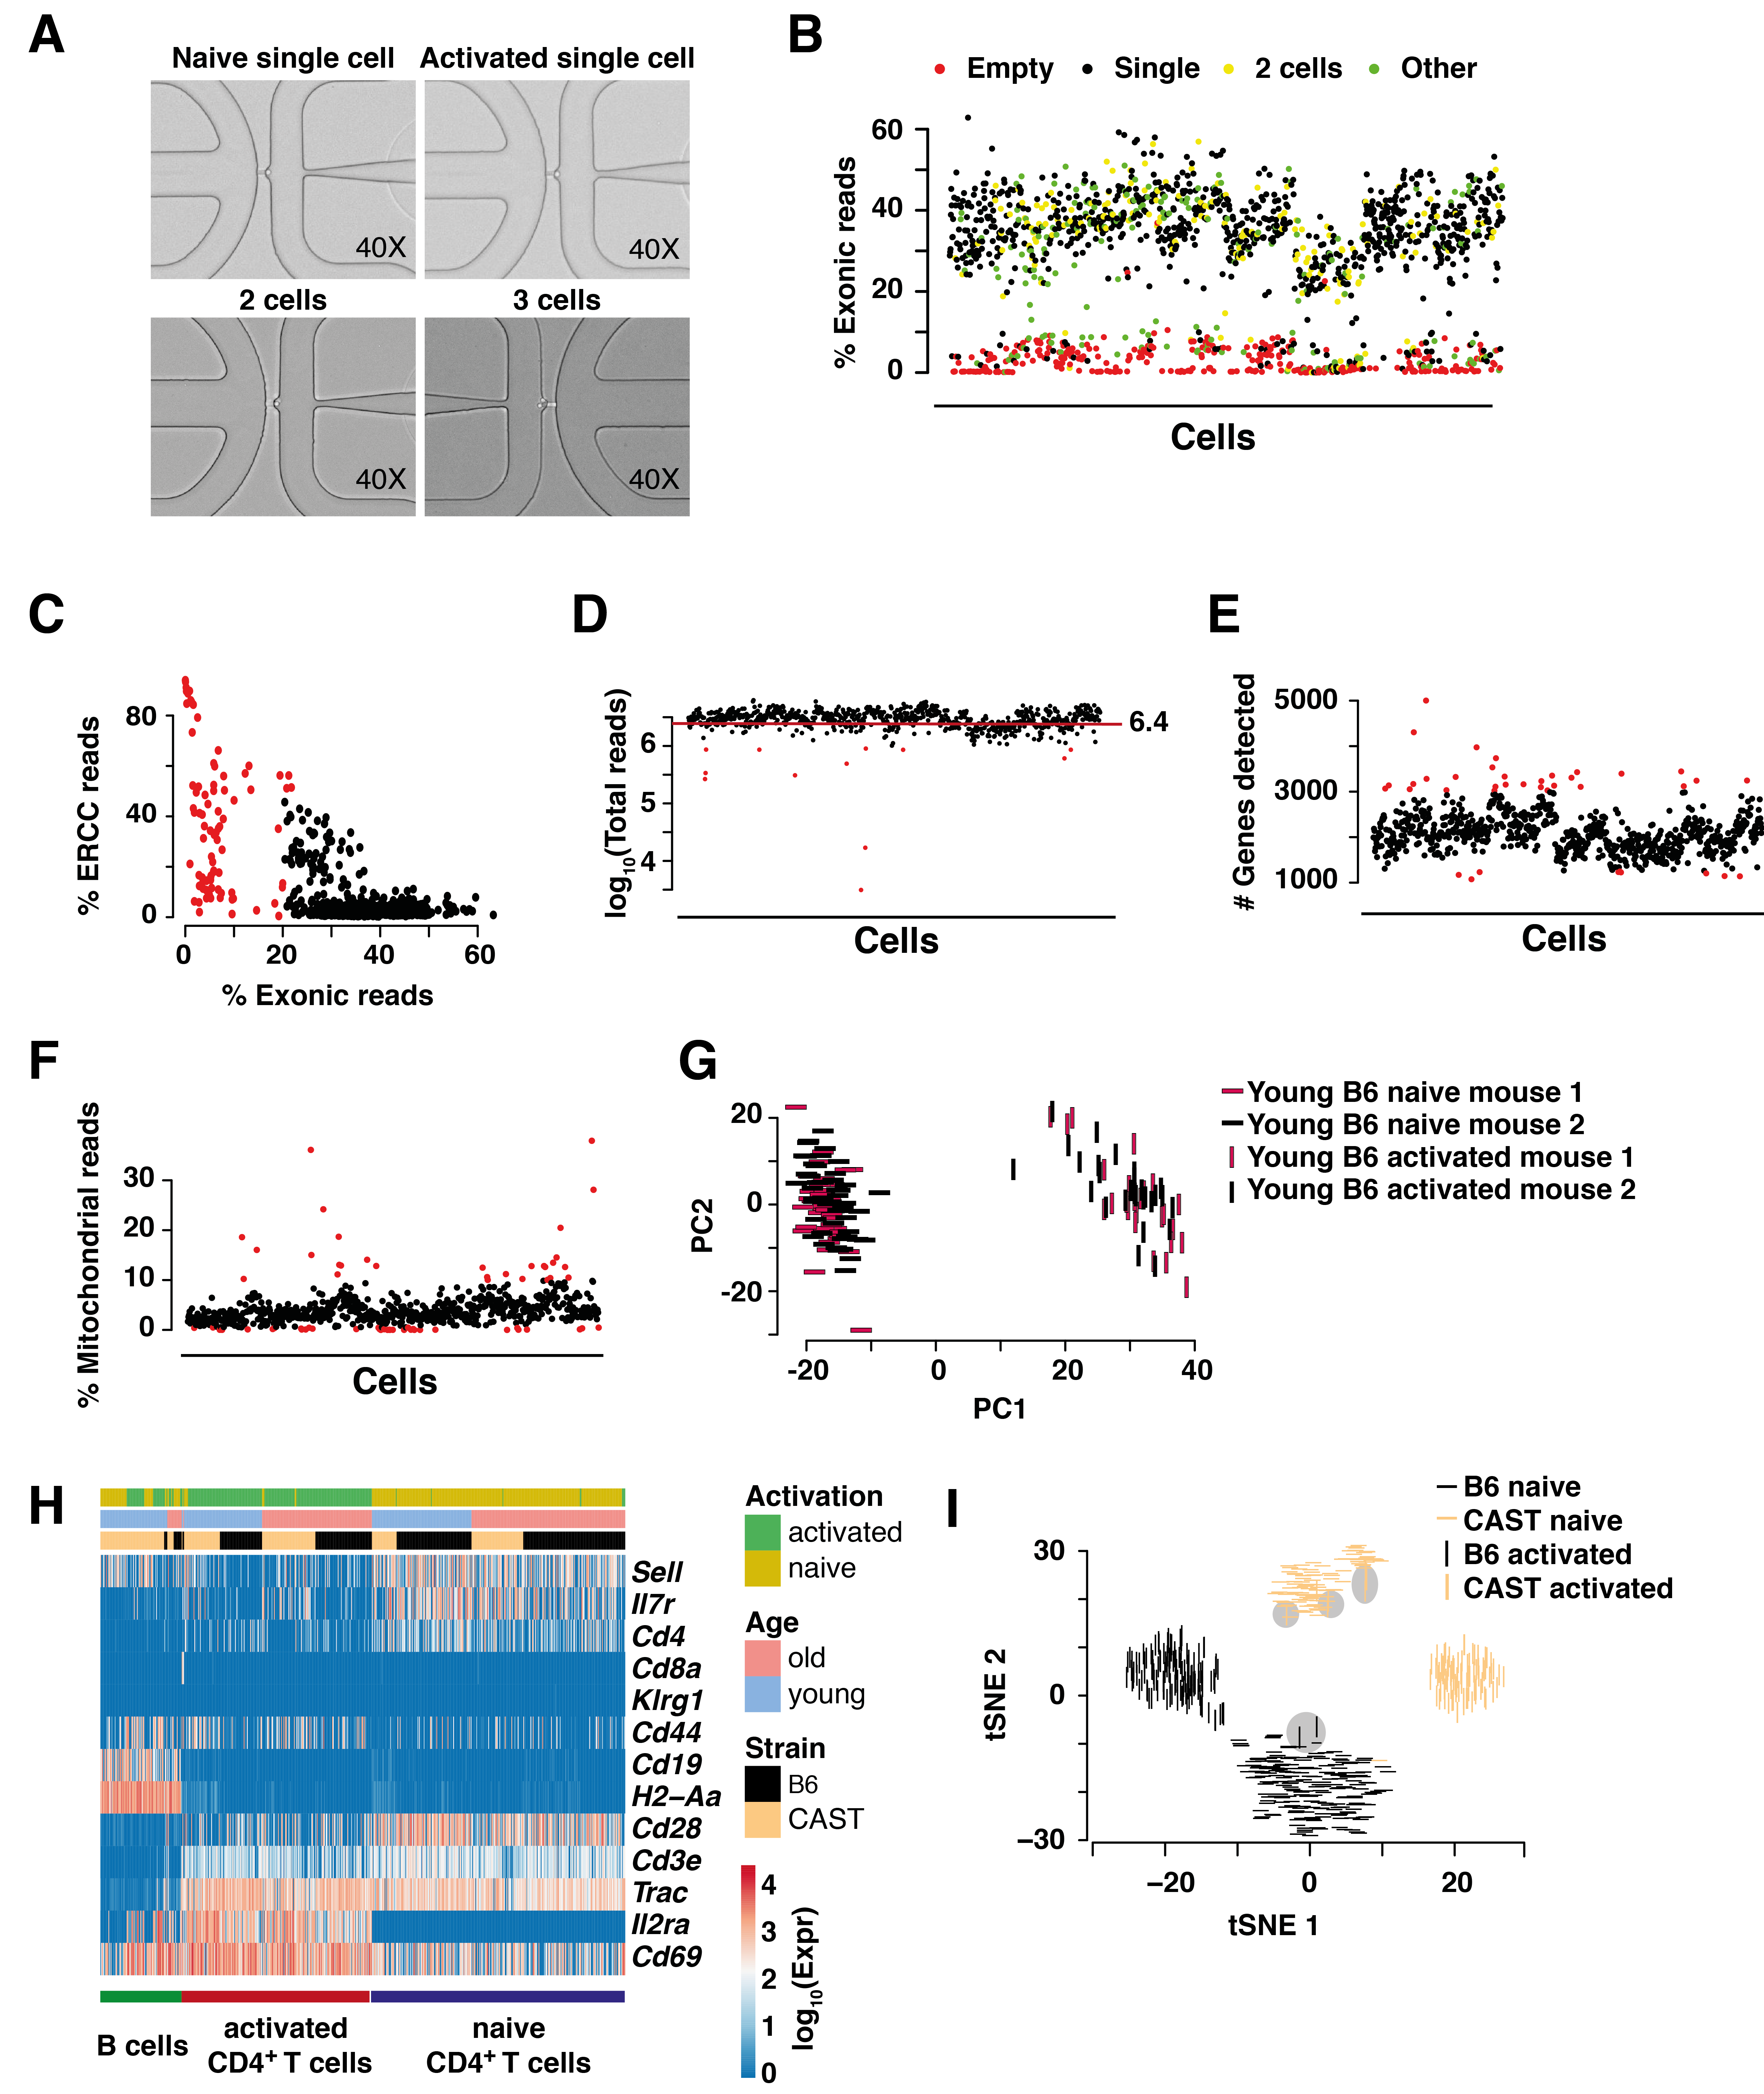
\includegraphics[width=0.9\textwidth]{Fig_3.png}
\caption[EFDR, FPR and TPR estimation using simulated data]{\textbf{EFDR, FPR and TPR estimation using simulated data (Full legend on next page).}\\
}\label{fig2:EFDR}
\end{figure}

\newpage

\captionsetup[figure]{list=no}
\addtocounter{figure}{-1}   
\captionof{figure}{\textbf{EFDR, FPR and TPR estimation using simulated data (continued).}\\
Data was simulated using the BASiCS model with model parameters set by empirical estimates based on on 98 microglia cells (see \textbf{Table \ref{tab2:datasets}}). Different samples sizes (40 - 200 cells) were simulated in replicates of 5. Differential testing was performed between 2 simulated datasets of equal size to calculate the false positive rate (FPR, number of detections divided by number of genes tested), the true positive rate (number of true positive divided by number of positives). Moreover, we report the expected false discovery rate (EFDR, \citep{Newton2004}). For each test, the EFDR was controlled to 10\% and the default minimum tolerance thresholds were used ($\tau_0 = \log_2(1.5)$, $\omega_0 = \log_2(1.5)$ and $\psi_0 = 0.41$), \textbf{(A)-(C)} Synthetic datasets generated using the null model (without changes in variability). FPR and EFDR for (A) differential mean expression, (B) differential over-dispersion and (C) differential residual over-dispersion testing using datasets with increasing samples sizes, \textbf{(D)-(E)} Synthetic datasets generated using the alternative model where 1000 genes were randomly selected and their associated over-dispersion parameters were increased or decreased by a $\log_2$ fold change of 5. TPR and EFDR for (D) differential over-dispersion testing and (E) differential residual over-dispersion testing using datasets with increasing samples sizes simulated.\\}
\captionsetup[figure]{list=yes}

As expected, the EFDR is controlled to 10\%. Furthermore, the FPR for differential mean expression and differential over-dispersion is consistently smaller than 10\% and is only slightly higher for differential residual over-dispersion testing. The TPR for differential over-dispersion and differential residual over-dispersion testing increases with increasing sample size and plateaus at 100\% \textbf{(Fig.~\ref{fig2:EFDR})}.

\subsection{Choice of hyper-parameters} \label{sec2:hyper-parameters}

As discussed above, the degrees of freedom $\eta$, the number of GRBFs  $L$ as well as their hyper-parameters ($m_l$, $h_l$) are set \emph{a priori}. Here, we explain the default values implemented in the extended BASiCS model. These were chosen to achieve a compromise between flexibility of the trend fit and the strength of shrinkage towards the estimated trend. Further discussion on the shrinkage can be found in \textbf{Section \ref{sec2:stabilization}}. \\ 

\todo{generate plots to show fits for different Ls and different cs.}\\

Firstly, we observed that large values of $L$ can lead to over-fitting but that small values of $L$ can limit the flexibility to capture non-linear relations between $\log(\delta_i)$ and $\log(\mu_i)$. Thus, as a parsimonious choice, we selected $L = 10$. Moreover, as in \cite{Kapourani2016}, values for $m_l$ were chosen to be equally spaced across the range of $\log(\mu_i)$:. 

\begin{equation} m_l = a + (l-1)\frac{b - a }{L-1}, \hspace{0.2cm}  l=1,\ldots, L, \end{equation} 

where $a=\min_{i\in\{1,\ldots,q_0\}}\{\log(\mu_i)\}$ and $b=\max_{i\in\{1,\ldots,q_0\}}\{\log(\mu_i)\}$. As $\mu_i$ values are unknown \emph{a priori} and change throughout the sampling procedure, $a$ and $b$ are updated every 50 MCMC iterations during the burn-in phase. Additionally, the scale hyper-parameters $h_l$ control the width of the GRBFs and, consequently, the locality of the regression. As a default, we set these as $h_l = c \times \Delta m$, where $c$ is a fixed proportionality constant and $\Delta m$ is the distance between consecutive values of $m_l$. In practice, we observed that the choice of a particular value of $c$ is not critical, as long as narrow kernels ($c<0.5$) are avoided. As a default, $c = 1.2$ was chosen. \\

The degrees of freedom $\eta$ controls the tails of the distribution for the residual term in \ref{eq::regression}. This influences the shrinkage towards the global trend and the robustness against outlying observations (here, these refer to genes whose mean and over-dispersion values are far from the trend).  If $\eta \geq 30$, $\epsilon_i$ approximately follows a normal distribution for which posterior inference for $\beta$ is known to be sensitive to outliers. Instead, small values of $\eta$ introduce heavy-tails for $\epsilon_i$, leading to more robust posterior inference. In principle, $\eta$ could be estimated within a Bayesian framework. However, this is problematic as the likelihood function associated to \ref{eq::regression} can be unbounded \citep{Fernandez1999}. Here, we opt for a pragmatic approach where the value of $\eta$ is fixed \emph{a priori}. To select a reasonable default value, we ran the regression BASiCS model for a grid of possible values of $\eta$ ($\eta \in \{ 1,2,3,4,5,6,7,8,9,15,20,25,30 \}$), using the datasets described in \textbf{Table \ref{tab2:datasets}} (with $L$, $m_l$ and $h_l$ fixed as described above). In all cases, we calculated a Monte Carlo estimates for the log-likelihood associated to \ref{eq::PoissonBASiCS} as a proxy for goodness-of-fit \textbf{Fig.~\ref{fig2:DoF}}. We observed that log-likelihood estimates were consistently the smallest for $\eta=1$ and that no substantial differences are observed across larger values of $\eta$. \\ 

\begin{figure}[!h]
\centering
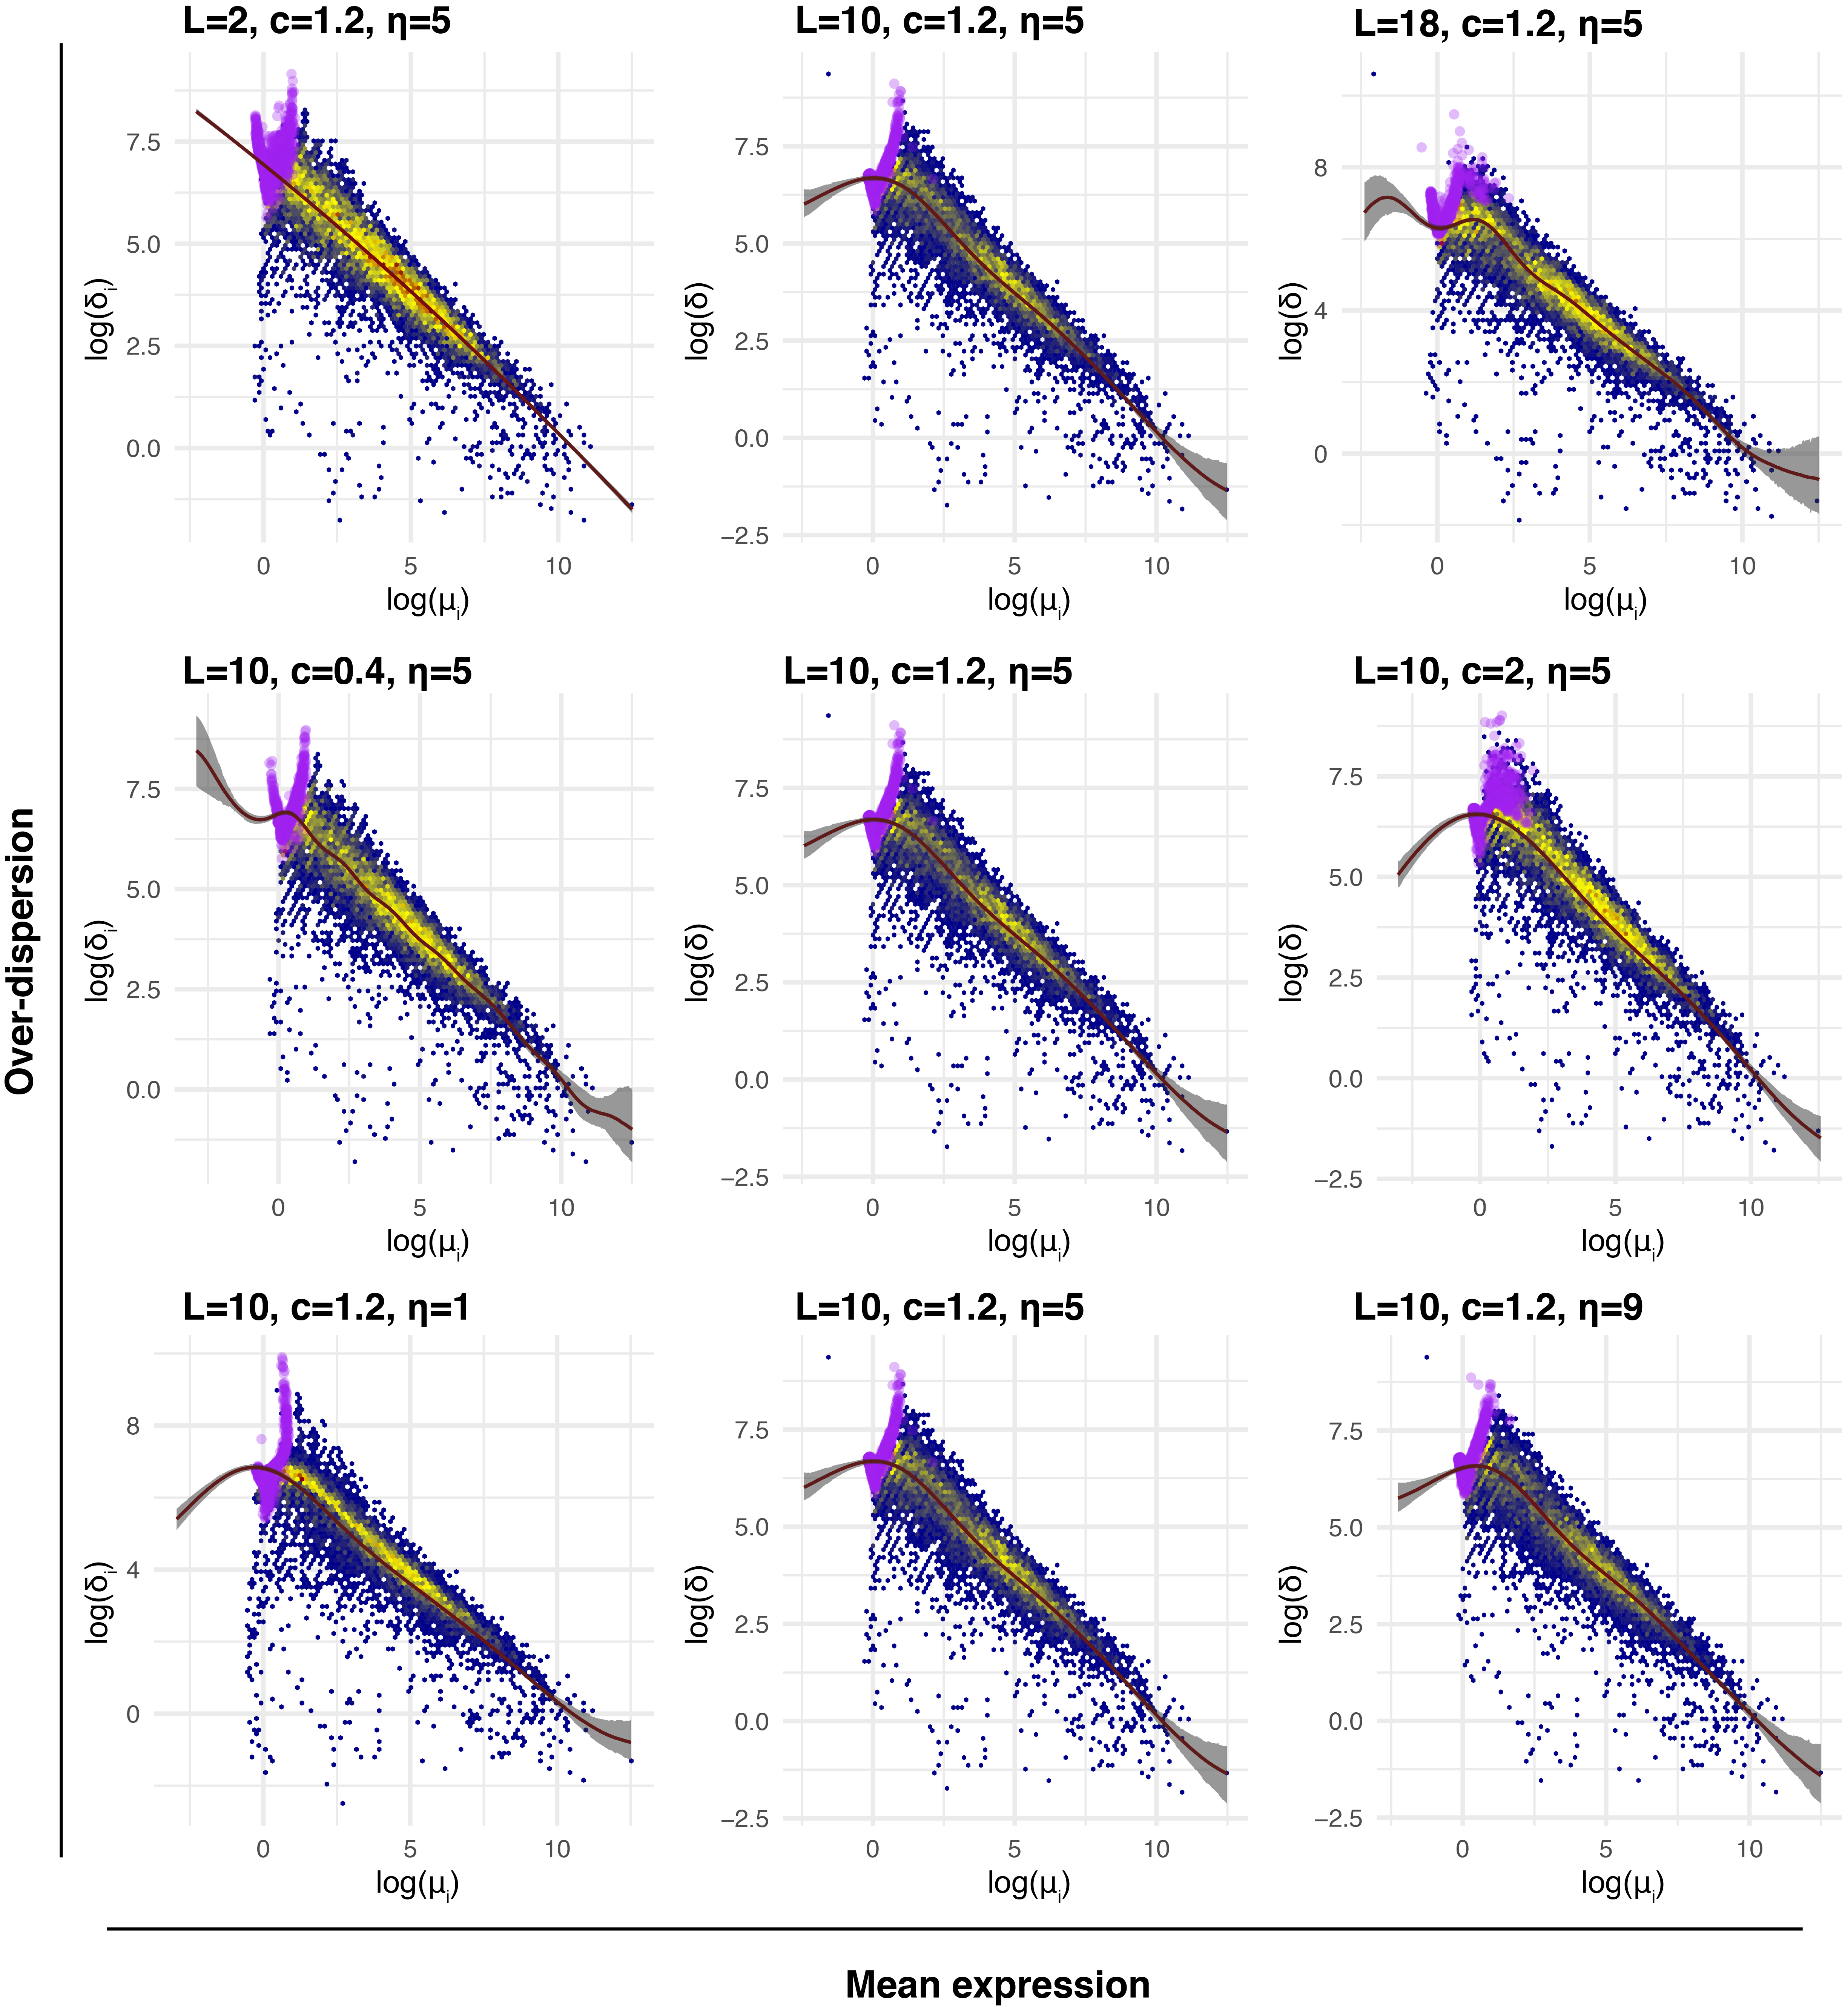
\includegraphics[width=\textwidth]{Fig_4.png}
\caption[Comparison of model fits for varying degrees of freedom]{\textbf{Comparison of model fits for varying degrees of freedom.}\\
\textbf{(A)} The regression BASiCS model was fit to datasets listed in Table \ref{tab2:datasets}. These include CA1 pyramidal neurons (CA1, \citep{Zeisel2015}), pool-and-split RNA 2i medium (PS, \citep{Grun2014}), mouse embryonic stem cells 2i medium (mESC, \citep{Grun2014}), Dictyostelium cells at day 0 of differentiation (Dict, \citep{Antolovic2017}) and naive CD4\plus{} T cells (CD4, \citep{Martinez-jimenez2017}). The model was fit using varying degrees of freedom and the log-likelihood was calculated as stated in equation \ref{eq::loglik}. The log-likelihood was scaled between the highest and lowest value for each dataset. \textbf{(B)} Posterior estimates of the variance parameter $\sigma^2$ depending on the number of degrees of freedom.}
\label{fig2:DoF}
\end{figure}

Based on these observations, default values implemented in the BASiCS software are set to $L=10, c=1.2, \eta=5$. Despite this, the model's implementation also allows flexible adjustment of $L$, $c$ and $\eta$ by the user. 

\section{Datasets used in this chapter} \label{sec2:datasets}

\subsection*{Quality filtering of single cell RNA sequencing data}
We employed a range of different datasets to test the proposed methodology. These datasets were selected to cover different experimental techniques (with and without unique molecular identifiers, UMI) and to encompass a variety of cell populations. Moreover, key features of each dataset can be found in \textbf{Table \ref{tab2:datatsets}}. 

\subsection{Dictyostelium cells} \label{seq::data_dict}

\cite{Antolovic2017} studied changes in expression variability between 0 hours (undifferentiated), 3 hours and 6 hours of \emph{Dictyostelium} differentiation. Raw data is available by direct download \citep[see Data S1 in][]{Antolovic2017}. Across all time-points, 5 cells were removed due to low quality. Technical spike-in genes that were not detected and biological genes with an average expression (across all cells) smaller than 1 count were removed. In total, 433 cells (131 cells and 3 batches at 0h, 157 cells and 3 batches at 3h, and 145 cells and 3 batches at 6h) and 10551 genes (88 technical and 10650 biological genes) passed filtering. We used data from the 0h time point to test the functionality of our model.

\subsection{Mouse brain cells} \label{seq::data_micro}
This dataset was composed of UMI scRNA-Seq data of cells isolated from the mouse somatosensory cortex and hippocampal CA1 region \citep{Zeisel2015}. Raw data is available from Gene Expression Omnibus under accession code GSE60361. 
Prior to the analysis, we removed technical genes with 0 total counts and biological genes for which the average count across all 3007 cells was below 0.1. The groups comprising microglia cells and CA1 neurons were chosen to be analysed. For these groups, 98 cells (microglia), 939 cells (CA1 pyramidal neurons) and 10744 genes (10687 biological and 57 technical genes) were left to be analysed.

\subsection{Pool-and-split RNAseq data} \label{seq::data_PaS}

This UMI-based dataset provides a control experiment to assess changes in biological heterogeneity in a situation where mean expression remains unchanged across conditions. Pool-and-split samples were created by pooling 1 million mESCs grown in 2i or serum medium and splitting 20pg of RNA into aliquots. These libraries are compared against single-cell samples (mESCs) \citep{Grun2014}. Raw data is available from Gene Expression Omnibus under accession code GSE54695. \\

As in \cite{Grun2014}, some cells were removed from the analysis due to low expression of the stem cell marker Oct4. Technical genes with 0 total counts were also removed from the analysis. Additionally, lowly expressed biological genes with fewer than 0.5 counts (on average, across all samples) were excluded. This left 258 libraries (74 single mESCs grown in 2i medium, 52 single mESCs grown in serum medium, 76 pool-and-split aliquots from cells grown in 2i medium and 56 pool-and-split aliquots from cells grown in serum medium) as well as 8924 genes (50 technical spike-ins and 8874 biological genes) for the analysis. Each condition contained 2 batches.\\

Matched single molecule florescence \textit{in situ} hybridization (smFISH) data from mESCs grown in 2i and serum media were obtained from Dominic Gr\"un (Max Planck Institute of Immunobiology and Epigenetics, Freiburg, Germany) through personal communications. This smFISH experiment assayed 9 genes (\textit{Gli1}, \textit{Klf4}, \textit{Notch1}, \textit{Pcna}, \textit{Pou5f1}, \textit{Sohlh2}, \textit{Sox2}, \textit{Stag3}, \textit{Tpx2}) in more than 70 cells per condition. We excluded \textit{Notch1} from the analysis due to strong disagreement between smFISH and scRNA-Seq data of cells grown in serum medium.

\subsection{CD4\plus{} T cells} \label{seq::data_cd4}

Non-UMI scRNA-Seq data of CD4\plus{} T cells were taken from \cite{Martinez-jimenez2017}. Raw data is available from ArrayExpress under accession code E-MTAB-4888. To perform a variety of tests, naive and activated CD4\plus{} T cells from young \emph{Mus musculus} (B6) mice were selected. Biological genes with an average count $<~1$ and non-detected technical genes were removed from the analysis. In total, 146 cells (93 naive and 53 activated CD4\plus{} T cells) and 10553 genes (10495 biological and 58 technical genes) passed filtering. Each condition contains 2 replicates.

\subsection{CD4\plus{} T cell differentiation} \label{seq::data_cd4diff}
Non-UMI scRNA-Seq data were generated from CD4\plus{} T cells during differentiation towards Th1 and Tfh cell fates after \emph{Plasmodium} infection \citep{Lonnberg2017}. Raw reads were downloaded from ArrayExpress [E-MTAB-4388] and mapped against the \emph{Mus musculus} genome (mm10) using \emph{gsnap} \citep{Wu2010a} with default settings. Read counting was performed using \emph{HTSeq} \citep{Anders2014} with default settings. \\

Quality control was performed by removing cells with fewer than 300,000 biological reads or fewer than 600,000 technical reads at day 2. At day 4 and 7, cells with fewer than 1,000,000 biological reads were excluded from downstream analysis. Additionally, we removed genes that did not show an average detection of more than 1 read at day 2, day 3, day 4 or day 7 after infection. After applying these criteria, 376 cells (Day 0: 16 cells, Day 2: 89, Day 3: 21, Day 4: 133, Day 7: 64, Day 7 non-infected: 53) and 7899 genes (7847 biological and 52 technical) remained for analysis. Note that, due to low sample sizes, we focused our analysis on data from day 2, day 4 and day 7 post-infection.

\newpage

\begin{table}[hb	]
\centering
\caption[Datasets used for model testing and novel analysis]{\textbf{Datasets used for model testing and novel analysis.} \\
For each of the datasets analysed in this study: number of cells (2$^{nd}$ column), number of genes (biological + technical spike-ins, 3$^{rd}$ column), number of batches (4$^{th}$ column), type of data acquisition system (5$^{th}$ column), information of whether the data was generated using unique molecular identifiers (UMIs, 6$^{th}$ column) and the reference to the original study (7$^{th}$ column) are provided.}
\label{tab2:datasets}
\begin{tabular}{lllllll}
\toprule
\textbf{Dataset} & \textbf{\# cells} & \textbf{\# genes} & \textbf{\# batches} & \textbf{Protocol} & \textbf{UMIs} & \textbf{Ref.}                       \\
\midrule
Young naive  & 93       & 10553    & 2          & Fluidigm C1       & No   & \citep{Martinez-jimenez2017} \\
CD4\plus{} T cells   &        &   &          &       & No   &  \\
\midrule

Young active    & 53       & 10553    & 2          & Fluidigm C1       & No   & \citep{Martinez-jimenez2017} \\
CD4\plus{} T cells    &        &     &           &        &    &  \\
\midrule

Microglia cells                         & 98       & 10687    & 1          & Fluidigm C1       & Yes  & \citep{Zeisel2015}           \\
\midrule

CA1 pyramidal                    & 948      & 10687    & 1          & Fluidigm C1       & Yes  & \citep{Zeisel2015}           \\
neurons       &       &     &           &       &   &           \\
\midrule

Malaria infected     & 89       & 7899     & 2          & Fluidigm C1       & No   & \citep{Lonnberg2017}         \\
CD4\plus{} T cells day 2     &        &      &          &  &    &  \\
\midrule

Malaria infected  & 133      & 7899     & 2          & Fluidigm C1       & No   & \citep{Lonnberg2017}         \\
CD4\plus{} T cells day 4     &       &      &    &  &    &\\
\midrule

Malaria infected  & 64       & 7899     & 1          & Fluidigm C1       & No   & \citep{Lonnberg2017}         \\
CD4\plus{}  T cells day 7    &   & &  &  &  &   \\
\midrule

Dictyostelium             & 131      & 10738    & 3          & Fluidigm C1       & No   & \citep{Antolovic2017}        \\
cells day 0  &  &   &   &  & & \\
\midrule

Pool-split RNA                 & 76       & 8924     & 2          & CEL-Seq           & Yes  & \citep{Grun2014}            \\
2i medium  &  &  & &  &  & \\
\midrule

mESC 2i medium    & 74       & 8924     & 2          & CEL-Seq           & Yes  & \citep{Grun2014} \\
\midrule

Pool-split RNA             & 56       & 8924     & 2          & CEL-Seq           & Yes  & \citep{Grun2014}            \\
serum medium &  &      &         &   &   &  \\
\midrule

mECS serum medium & 52       & 8924     & 2          & CEL-Seq           & Yes  & \citep{Grun2014} \\
\bottomrule       
\end{tabular}
\end{table}


\section{The informative prior stabilizes parameter estimation}
\label{sec2:stabilization}

Our joint prior formulation has introduced a non-linear regression to capture the overall trend between gene-specific over-dispersion parameters $\delta_i$ and mean expression parameters $\mu_i$. Thus, we also refer to the extended model induced by this prior as the \textit{regression} BASiCS model. Accordingly, the model induced by the original independent prior specification \citep{Vallejos2016} is referred to as the \textit{non-regression} BASiCS model.\\ 

To study the performance of the regression BASiCS model, we applied it to a variety of scRNA-Seq datasets. Each dataset is unique in its composition, covering a range of different cell types and experimental protocols (see section \ref{sec2:datasets} and \textbf{Table \ref{tab2:datatsets}}). Qualitatively, we observe that the inferred regression trend varies substantially across different datasets \textbf{(Fig.~\ref{fig2:datasets}}, justifying the choice of a flexible semi-parametric approach (see section \ref{sec2:extended_BASiCS} and section \ref{sec2:hyper-parameters}). Moreover, as expected, we observe that residual over-dispersion parameters $\epsilon_i$ are not confounded by mean expression, nor by the percentage of zero counts per gene \textbf{(Fig.~\ref{fig2:datasets}}. \\

\newpage

\begin{figure}[!h]
\centering
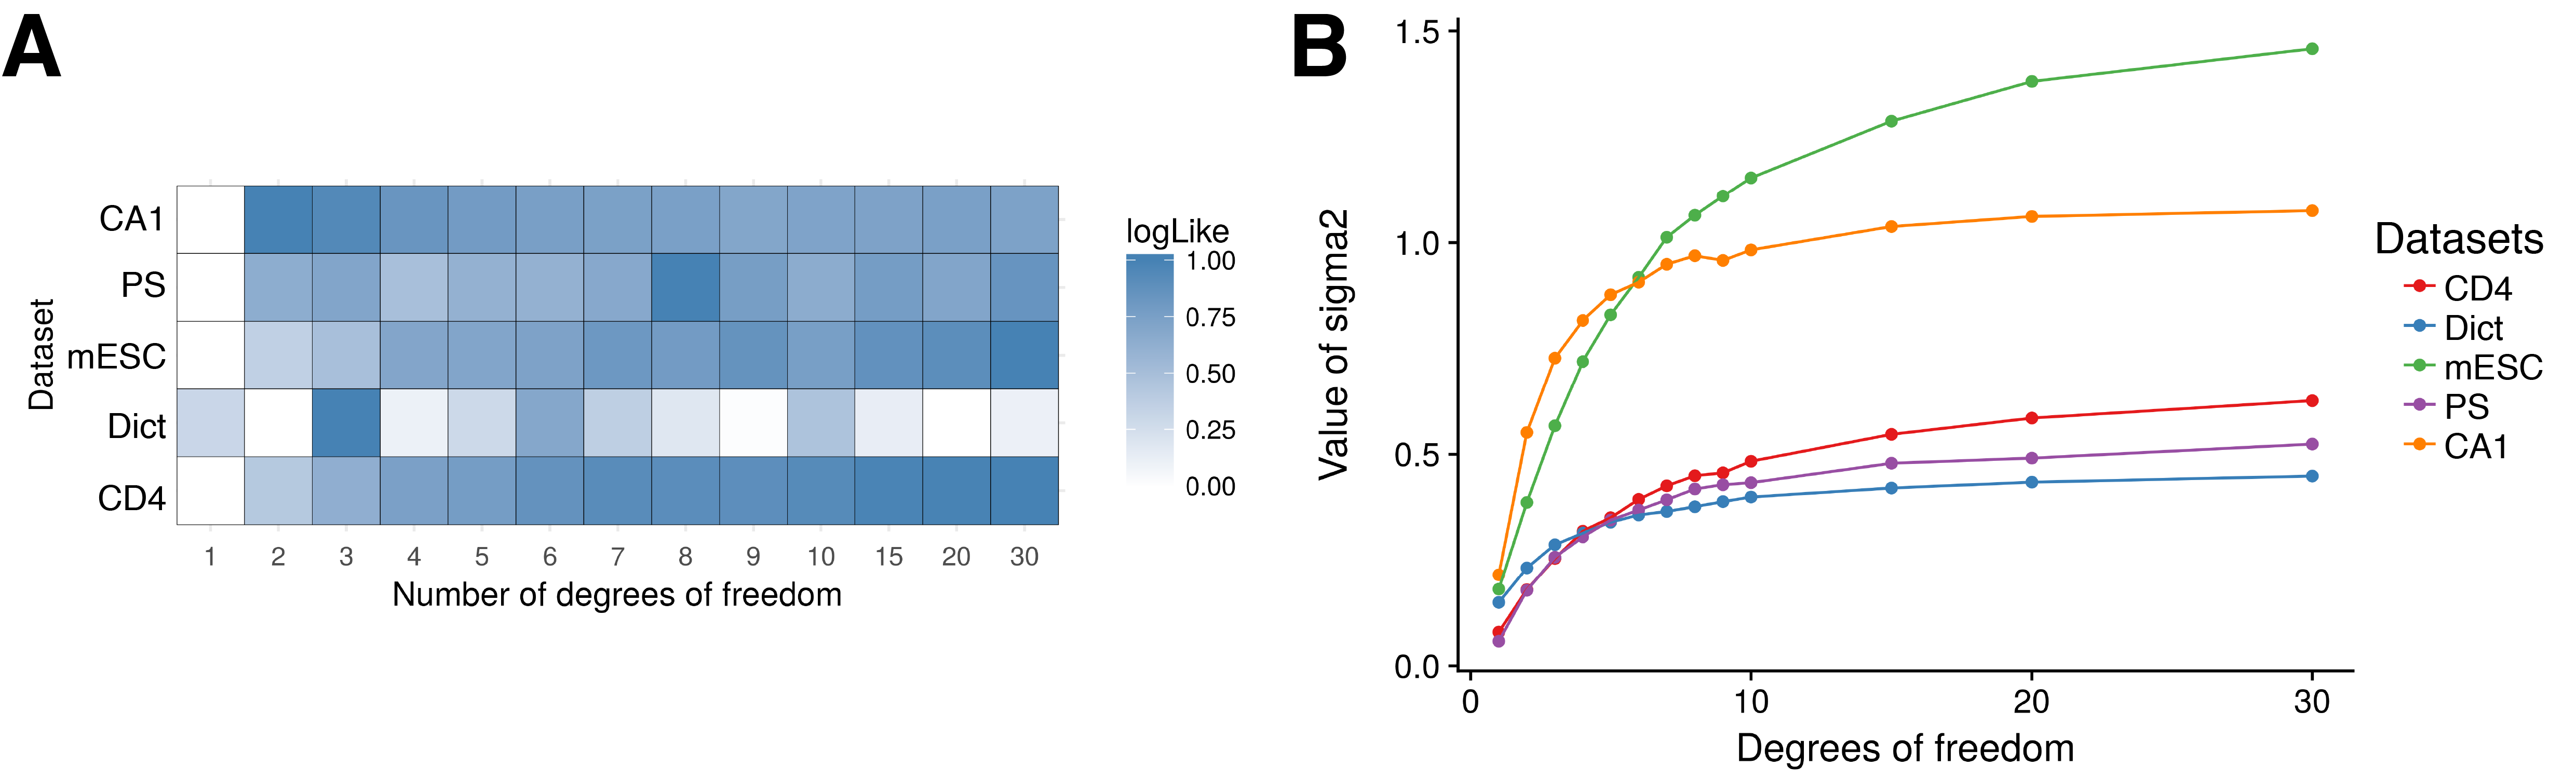
\includegraphics[width=0.95\textwidth]{Fig_5.png}
\caption[Parameter estimation using a variety of scRNA-Seq datasets]{\textbf{Parameter estimation using a variety of scRNA-Seq datasets.}\\
Model parameters were estimated using the regression and non-regression BASiCS models on \textbf{(A)} naive CD4\plus{} T cells \citep{Martinez-jimenez2017}, \textbf{(B)} \textit{Dictyostelium} cells prior to differentiation (day 0) \citep{Antolovic2017}, \textbf{(C)} microglia cells \citep{Zeisel2015} and \textbf{(D)} pool-and-split RNA \citep{Grun2014}. These datasets were selected to highlight two situations with different levels of sparsity (i.e.~the proportion of zero counts, see fourth column). The colour code within the scatterplots is used to represent areas with high (yellow/red) and low (blue) concentration of genes. \textbf{First column:} gene-specific over-dispersion $\delta_i$ versus mean expression $\mu_i$ as estimated by the non-regression BASiCS model.\textbf{Second column:} gene-specific over-dispersion $\delta_i$ versus mean expression $\mu_i$ as estimated by the regression BASiCS model. The red line indicates the estimated regression trend. Purple dots indicate genes detected (i.e. with at least one count) in less than 2 cells. \textbf{Third column:} gene-specific residual over-dispersion $\epsilon_i$ versus mean expression $\mu_i$ as estimated by the regression BASiCS model. \textbf{Forth column:} gene-specific posterior estimates for residual over-dispersion $\epsilon_i$ parameters versus percentage of zero counts for each gene.\\}
\label{fig2:datasets}
\end{figure}

\newpage

The regression BASiCS model introduces a joint prior specification for $(\mu_i, \delta_i)'$, shrinking the posterior estimates for $\mu_i$ and $\delta_i$ towards the regression trend [this is in line with the shrinkage observed in Love et al. \citep{Love2014}]. The strength of this shrinkage is dataset-specific, being more prominent in sparser datasets with a higher frequency of zero counts \textbf{(Fig.~\ref{fig2:datasets}A)} and for lowly-expressed genes where measurement error is greatest. \\

\begin{figure}[!h]
\centering
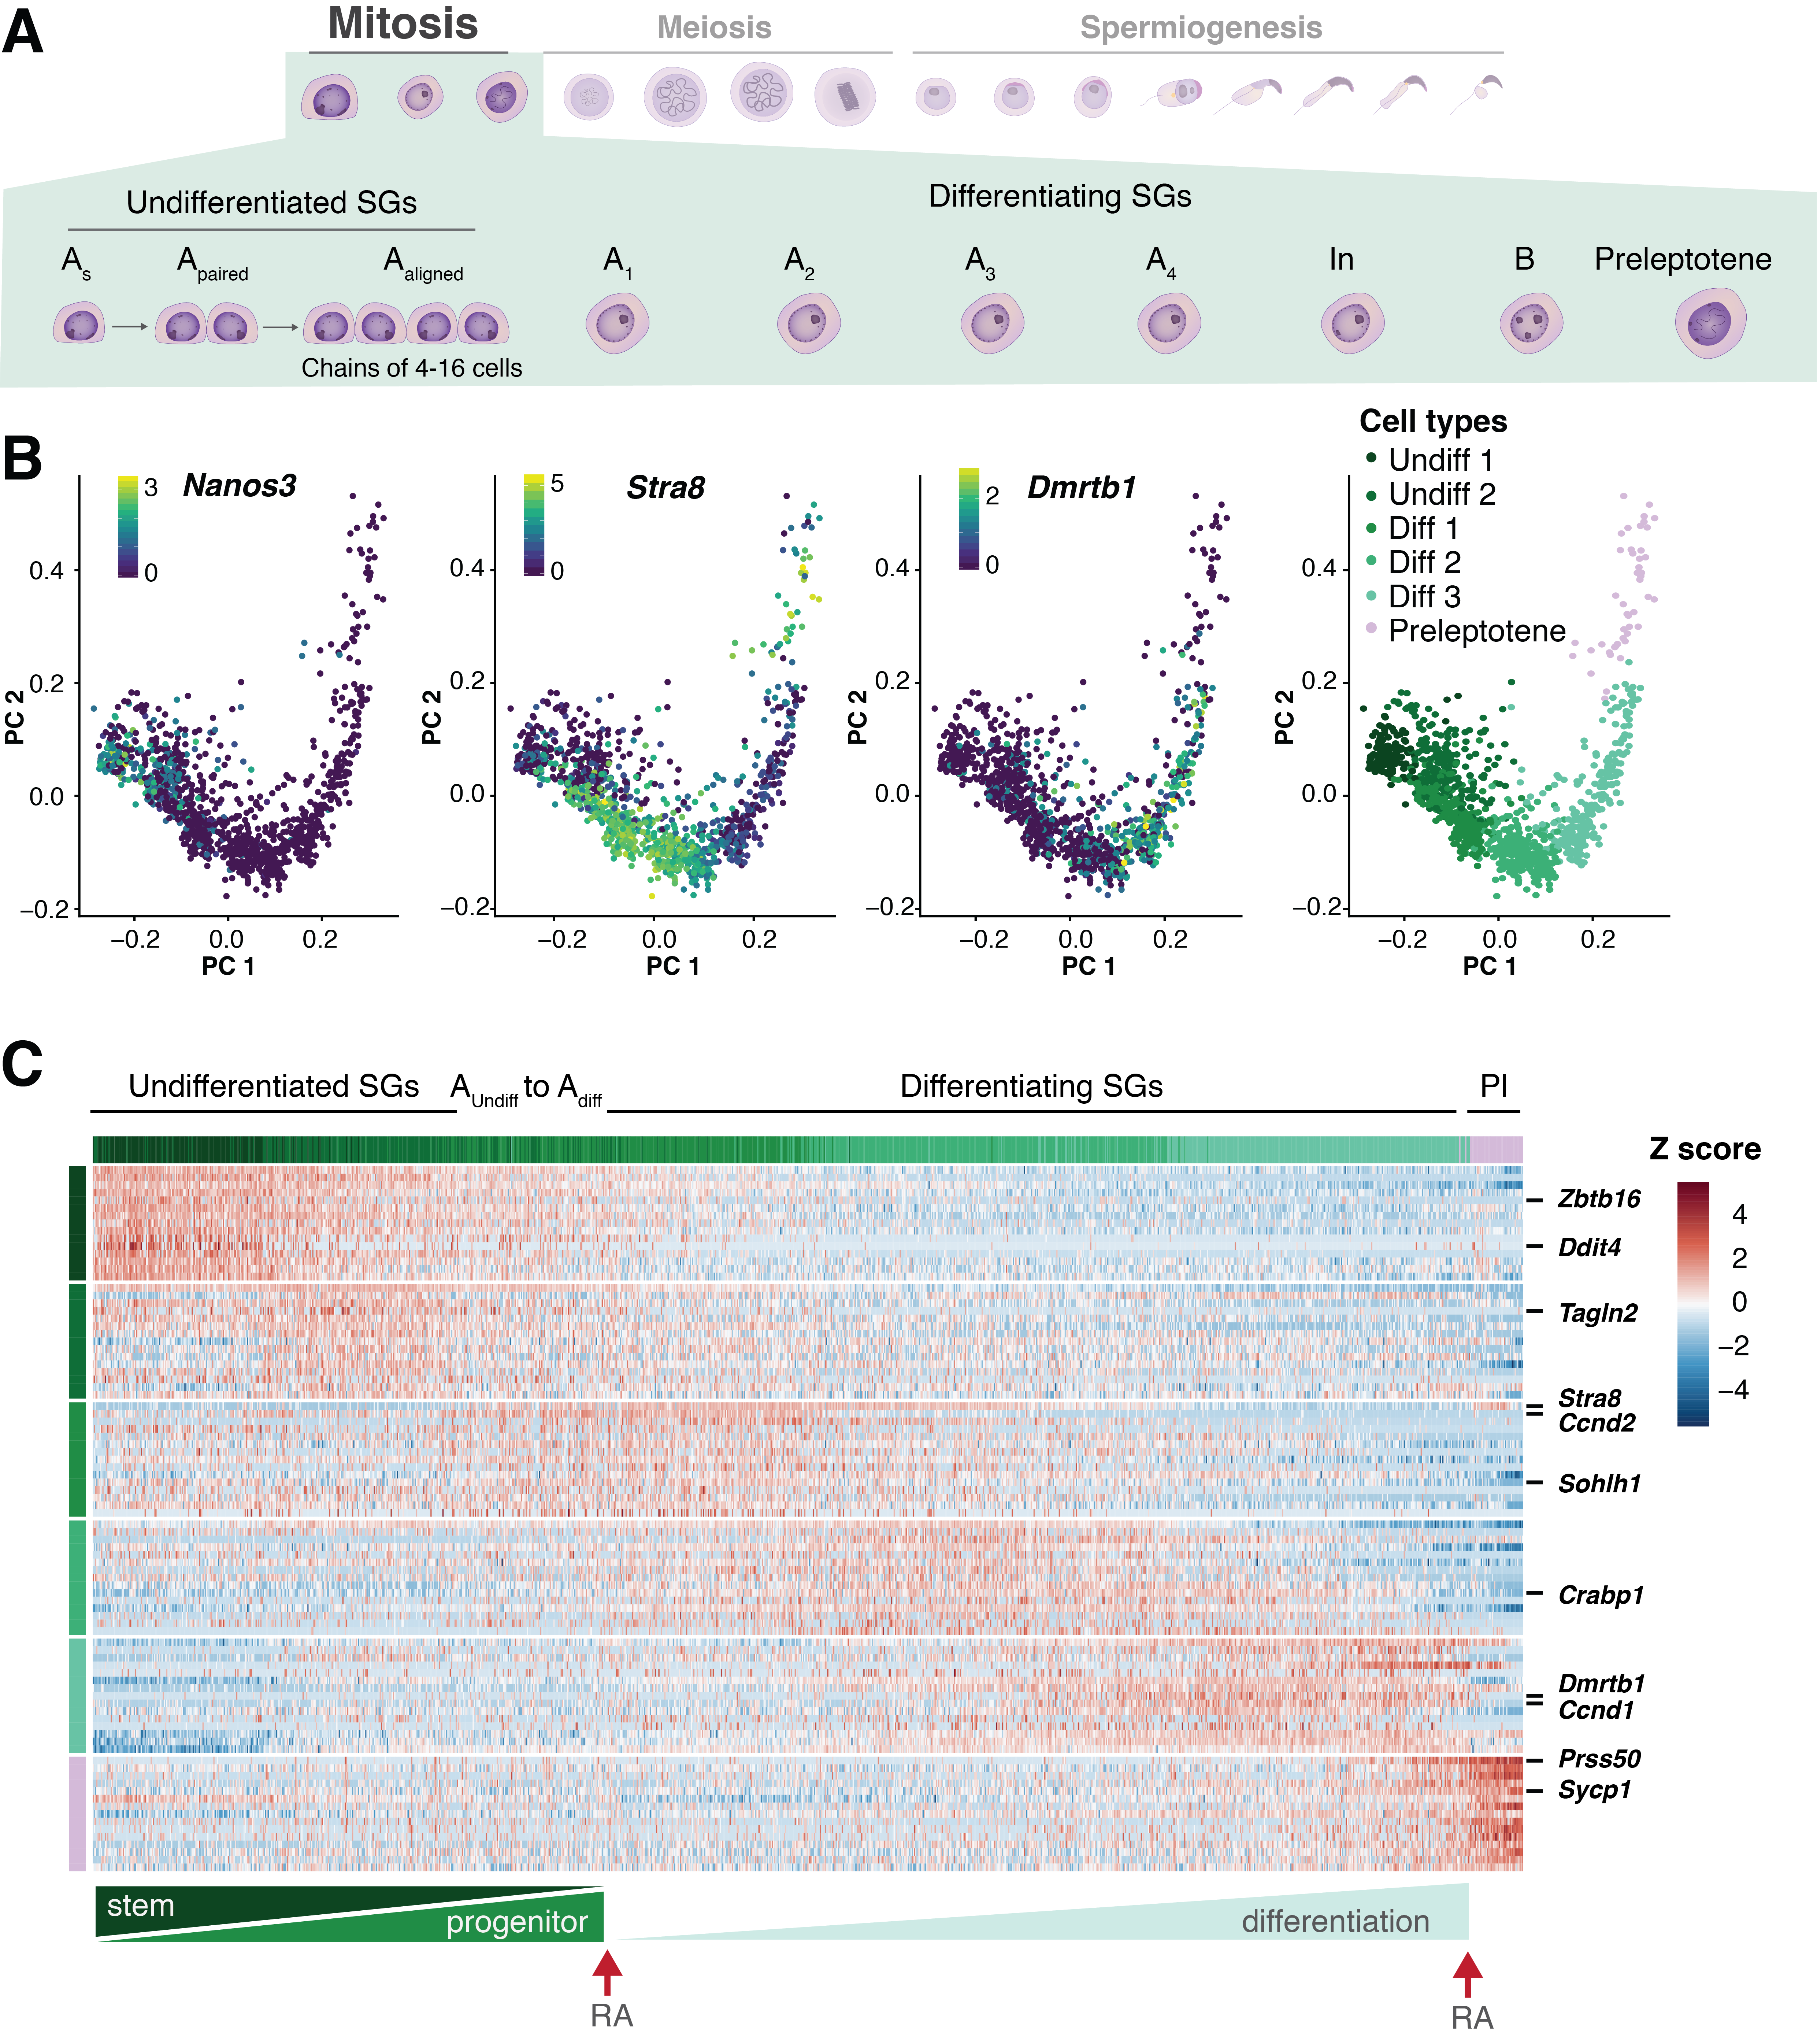
\includegraphics[width=\textwidth]{Fig_6.png}
\caption[Estimation of gene-specific model parameters for varying sample sizes]{\textbf{Estimation of gene-specific model parameters for varying sample sizes.}\\
The regression (orange) and non-regression (blue) BASiCS models were used to estimate gene-specific model parameters for lowly (lower panels), medium (mid panels) and highly (upper panels) expressed genes across populations with varying numbers of cells. These were generated by randomly sub-sampling cells from a population of 939 CA1 pyramidal neurons \citep{Zeisel2015}. Extended results based on multiple downsampling experiments are displayed in \textbf{Fig.~\ref{fig2:parameter_stabilization2}}.  \\
\textbf{(A-C)} For a single sub-sampling experiment, boxplots summarize the distribution of gene-specific estimates for (A) mean expression parameters $\mu_i$ (log-scale), (B) over-dispersion parameters $\delta_i$ (log-scale) and (C) residual over-dispersion parameters $\epsilon_i$.}
\label{fig2:parameter_stabilization}
\end{figure}

Subsequently, we asked whether or not the shrinkage introduced by the regression BASiCS model improves posterior inference. To assess this, we compared estimates for gene-specific parameters across: (i) different sample sizes and (ii) different gene expression levels. More concretely, we used a large dataset containing 939 CA1 pyramidal neurons \citep{Zeisel2015} to artificially generate smaller datasets by randomly sub-sampling 50-500 cells. For each sample size, parameter estimates were then obtained using both the regression and non-regression BASiCS models. 
Based on parameter estimates using the non-regression model, we split the genes into three sets: lowly expressed ($\mu_i<1.89$), medium expressed ($1.89<\mu_i<5.37$) and highly expressed ($\mu_i>5.37$). These cut-off values were chosen such that a third of genes classifies into each category. The distribution of these estimates is summarised in \textbf{Fig.~\ref{fig2:parameter_stabilization}}. \\

Firstly, we observe that both the regression and non-regression BASiCS models led to comparable and largely stable mean expression estimates across different sample sizes and expression levels \textbf{(Fig.~\ref{fig2:parameter_stabilization}A)}. Secondly, in line with the results in \textbf{Fig.~\ref{fig2:datasets}}, the main differences between the methods arise when estimating the over-dispersion parameters $\delta_i$ \textbf{(Fig.~\ref{fig2:parameter_stabilization}B and \ref{fig2:parameter_stabilization2}A-C)}. In particular, we observe that the non-regression BASiCS model appears to underestimate $\delta_i$ for lowly expressed genes when the sample size is small (with respect to the parameter estimates obtained based on the full dataset of 939 cells). In contrast, the shrinkage introduced by our regression BASiCS model aids parameter estimation, leading to robust estimates even for the smallest sample size. This is particularly important for rare cell populations where large sample sizes are difficult to obtain. A similar effect is observed for genes with medium and high expression levels, where the non-regression BASiCS model appears to overestimate $\delta_i$. We also observe that estimates of residual over-dispersion parameters $\epsilon_i$ are stable across sample sizes and expression levels. \textbf{Fig.~\ref{fig2:parameter_stabilization2}D-F} summarizes 10 replicates of the downsampling experiment performed in \textbf{Fig.~\ref{fig2:parameter_stabilization}A-C}. For each sub-sampling experiment, sample size and gene set, we computed the median $\log_2$ fold change in $\mu_i$ and $\delta_i$ and the median difference for $\epsilon_i$ between estimates and the \emph{pseudo} ground truth. The median and the range of these values across 10 sub-sampling experiment is used for visualization purposes \textbf{(Fig.~\ref{fig2:parameter_stabilization2}D-F)}. \\

As an external validation, we compared our posterior estimates of gene-specific model parameters obtained from scRNA-Seq data to empirical estimates from matched smFISH data of mouse embryonic stem cells grown in 2i and serum media \citep{Grun2014}. Firstly, posterior estimates of mean-expression parameters $\mu_i$ exhibit high correlation to smFISH mean transcript counts \textbf{(Fig.\ref{fig2:parameter_stabilization2}G)}. Secondly, we also observe a strong correlation between posterior estimates for over-dispersion parameters $\delta_i$ and the empirical CV$^2$ values obtained from smFISH data \textbf{(Fig.\ref{fig2:parameter_stabilization2}H)}. Finally, a similar behaviour is observed when comparing posterior estimates of residual over-dispersion parameters $\epsilon_i$ to a residual CV$^2$ \textbf{(Fig.\ref{fig2:parameter_stabilization2}I)}. As in \cite{Brennecke2013}, to obtain residual CV$^2$ values for the smFISH data, we fitted a gamma generalized linear model with identity link (\textit{glmgam.fit} of the \textit{statmod} package in R) between the CV$^2$ and the reciprocal log-transformed mean transcript counts.


\begin{figure}[!h]
\centering
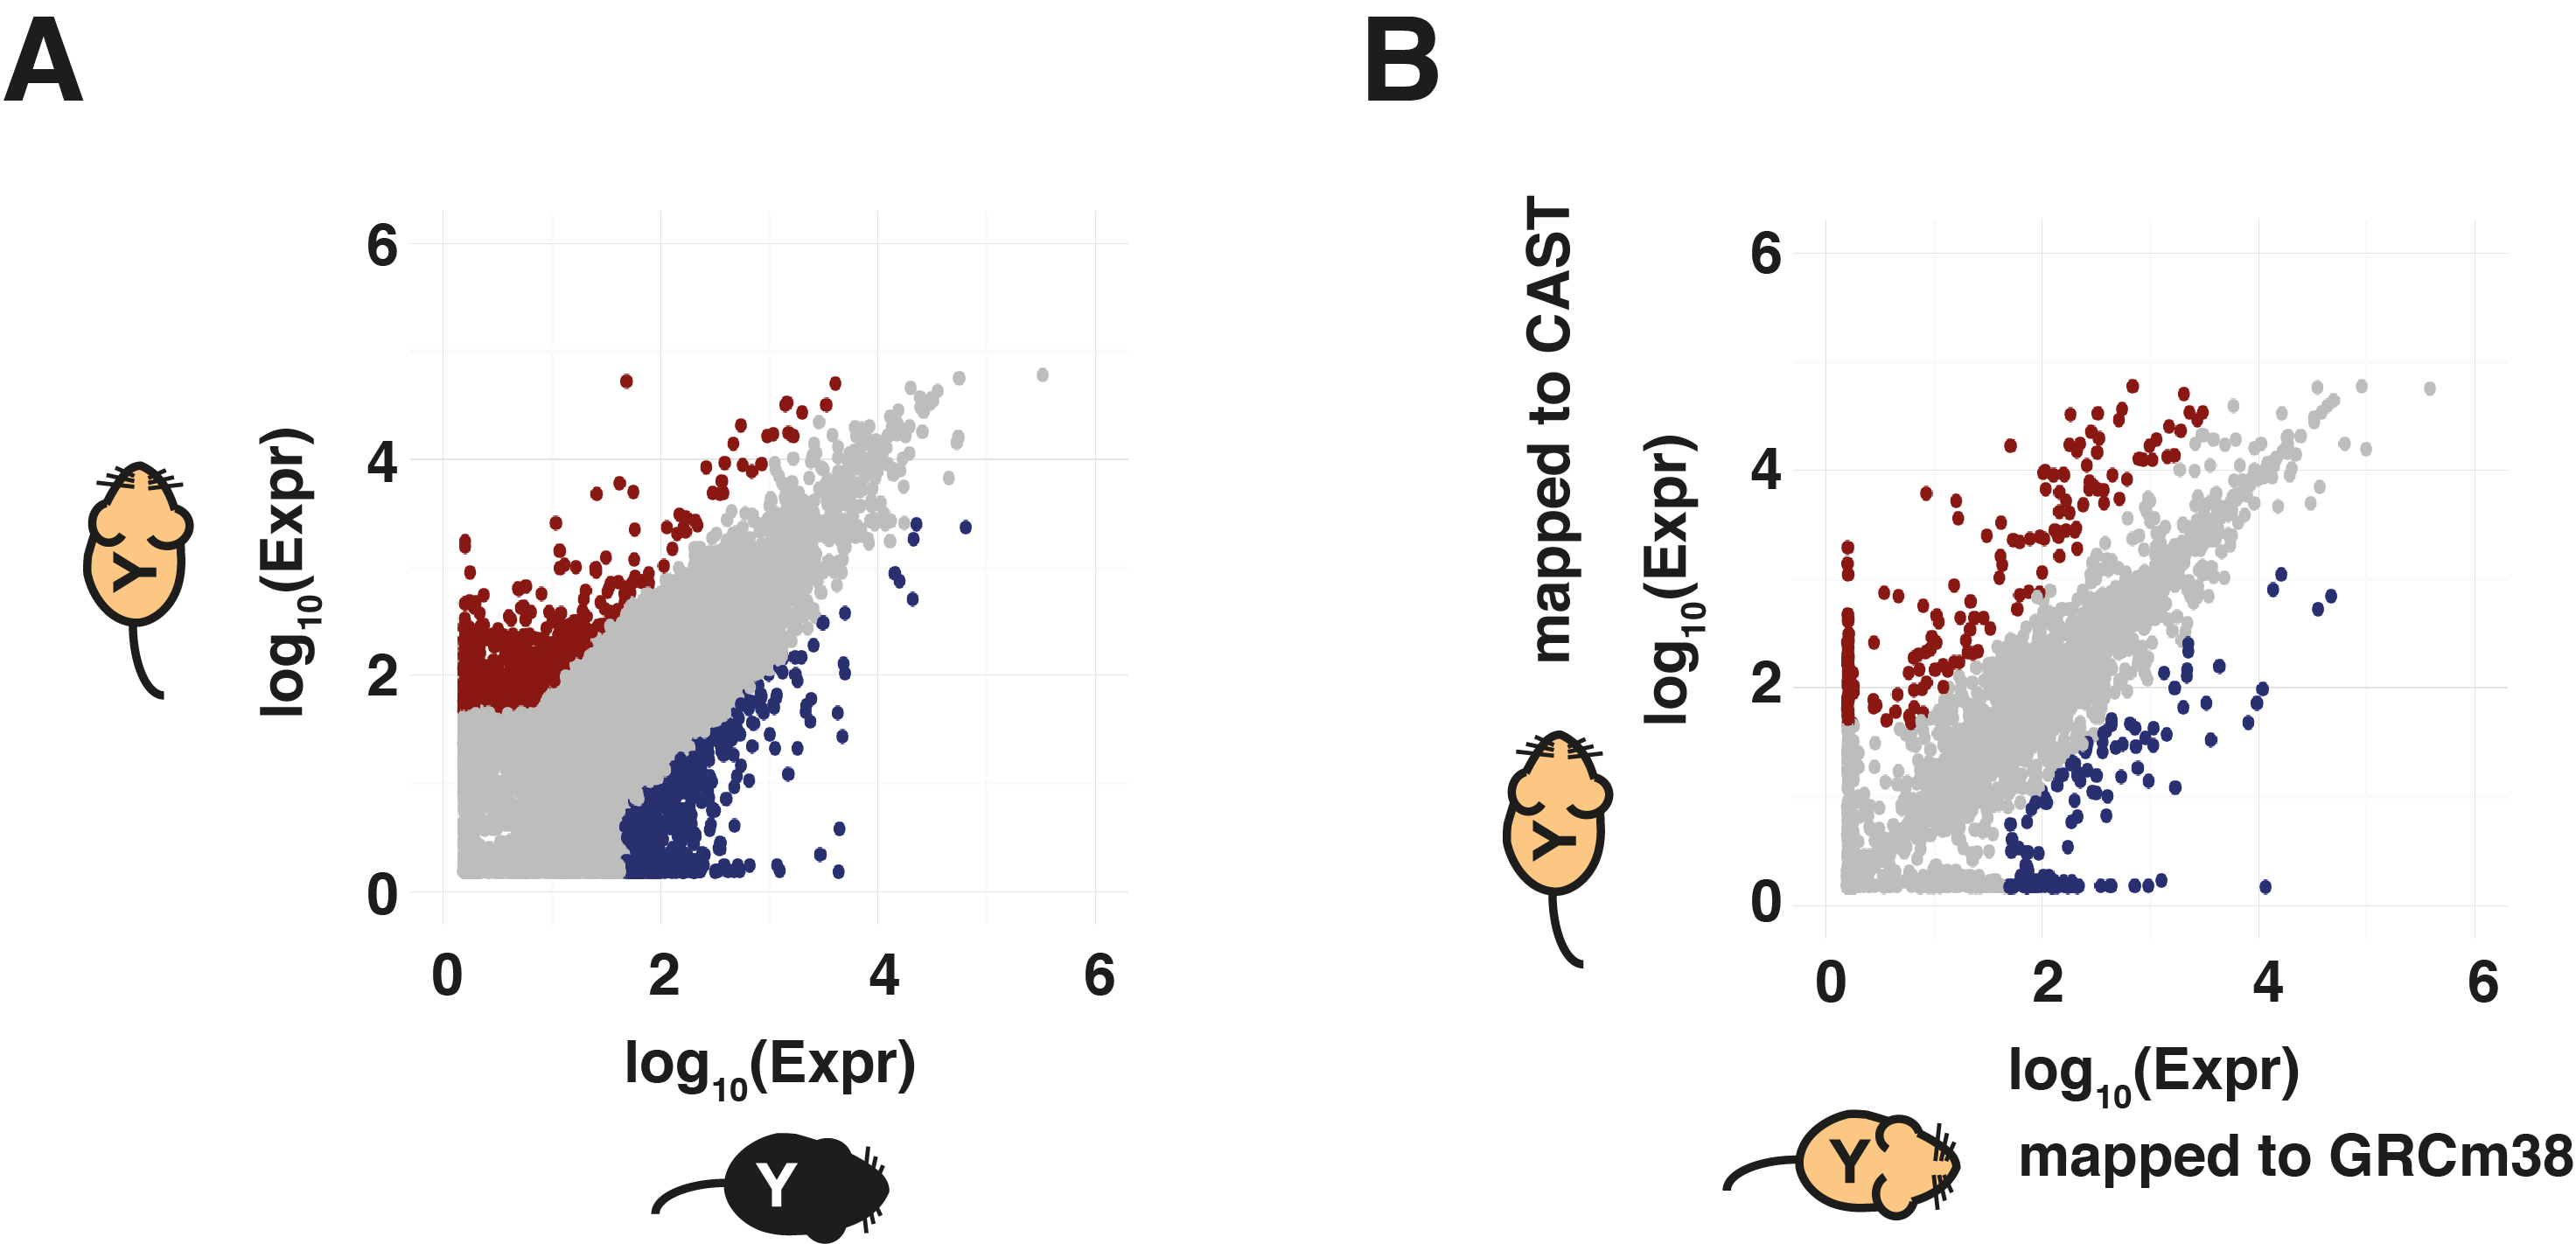
\includegraphics[width=0.9\textwidth]{Fig_7.png}
\caption[Stability of posterior estimates for gene-specific parameters]{\textbf{Stability of posterior estimates for gene-specific parameters.}\\
\textbf{(A-C)} The regression and non-regression BASiCS models were used to estimate gene-specific model parameters for three difference sample sizes: (A) 50 cells, (B) 250 cells and (C) 939 cells. The cells used in (A) and (B) were randomly sampled from the full population of 939 pyramidal CA1 neurons \citep{Zeisel2015}. The log$_2$ fold change in over-dispersion estimates between the regression and non-regression BASiCS models (vertical axis) is plotted against overall mean expression (horizontal axis). The colour code within the scatterplots is used to represent areas with high (yellow/red) and low (blue) concentration of genes. \textbf{(D-F)} The regression (orange) and non-regression (blue) BASiCS models were used to estimate gene-specific model parameters for lowly (lower panels), medium (mid panels) and highly (upper panels) expressed genes across populations with varying numbers of cells. These were generated by randomly sub-sampling cells from a population of 939 pyramidal CA1 neurons \citep{Zeisel2015}. For 10 sub-sampling experiments, parameter estimates were compared against a \textit{pseudo} ground truth (pgt). The latter is defined as the parameter estimates obtained for the full population of 939 cells using the regression BASiCS model. For each sub-sampling experiment, gene-specific log$_2$ fold changes ($\log_2(\mu_i/\mu_{i,pgt})$ and $\log_2(\delta_i/\delta_{i,pgt})$) and distances ($\epsilon_i - \epsilon_{i,pgt}$) between the estimates and the pgt were computed. For visualisation purposes, the medians across genes for each sub-sampling experiment are presented. }
\label{fig2:parameter_stabilization2}
\end{figure}

\newpage

\captionsetup[figure]{list=no}
\addtocounter{figure}{-1}   
\captionof{figure}{\textbf{Stability of posterior estimates for gene-specific parameters (continued).}\\
\textbf{(G-I)} Matched scRNA-Seq and smFISH data measured on mouse embryonic stem cells grown in 2i and serum media \citep{Grun2014} was used to validate the performance of the regression BASiCS model. Gene-specific parameter estimates obtained by the regression BASiCS model were compared against empirical estimates calculated based on smFISH data. This comparison includes 8 genes, measured in both conditions. Pearson's correlation is indicated for each comparison. \textbf{(G)} Estimates of mean expression parameters $\mu_i$ (log-scale) are plotted against mean transcript count (smFISH). \textbf{(H)} Estimates of over-dispersion parameters $\delta_i$ (log-scale) are plotted against the squared coefficient of variation (CV$^2$) of transcript counts (smFISH). \textbf{(I)} Estimates for residual over-dispersion parameters $\epsilon_i$ are compared against residual estimates of variability estimated for the smFISH data.\\}
\captionsetup[figure]{list=yes}

\section{Expression variability dynamics during immune responses}

Here, we illustrate how our method assesses changes in expression variability using CD4\plus{} T cells as model system. For all datasets, pre-processing steps are described in section \ref{sec2:datasets}. 

\subsection{Testing variability changes upon immune activation}

We extended the BASiCS framework to assess changes in variability even for genes that change in mean expression. This was not possible for the analysis done on the previous chapter. We therefore extend the previous analysis including the full set of expressed genes. \\

To identify gene expression changes during early T cell activation, we compared CD4\plus{} T cells before (naive) and after (active) 3 hours of stimulation \citep{Martinez-jimenez2017}. When using the non-regression BASiCS model, our differential over-dispersion test avoided the confounding with mean expression by solely focusing on genes with no changes in mean expression. This represents only a small fraction 
out of the full set of expressed genes. In contrast, testing changes in variability through residual over-dispersion allows testing across all genes, including the large set of genes that are up-regulated upon immune activation \textbf{(Fig.~\ref{fig1:immune_activation} and Box 2)}. The latter include immune-response genes and critical drivers for CD4\plus{} T cell functionality.\\

Firstly, we compare the results obtained by the regression BASiCS model with respect those presented in section \ref{sec1:Tcell_activation}.  
To allow a direct comparison of the results, the same inclusion criteria as in section \ref{sec1:Tcell_activation} is adopted, i.e.~we excluded genes with low mean expression ($\mu_i<50$) in both conditions from testing. Moreover, our  minimum tolerance thresholds were also adapted to match the choices in section \ref{sec1:Tcell_activation}. To detect differentially expressed genes (mean) a minimum tolerance threshold $\tau_0 = 2$ was used \textbf{(Fig.~\ref{fig2:model_comparison}A)}. To compare the detection of differentially over-dispersed genes, we performed differential mean expression testing using a stringent minimum tolerance threshold $\tau_0 = 0$ for both models (this is to avoid the results to be confounded by changes in mean, see upper panel in \textbf{Fig.~\ref{fig2:model_comparison}B}). For the 463 genes that are detected as non-differentially expressed by both models for this threshold, a total of 111 genes are detected as differentially over-dispersed by either model (minimum tolerance log$_2$ fold change threshold $\omega_0 = \log_2(1.5) = 0.58$). Out of this set, 93 genes ($\sim$83\%) are detected as differentially over-dispersed by both models (see lower panel in \textbf{Fig.~\ref{fig2:model_comparison}B}). \\

\begin{figure}[!h]
\centering
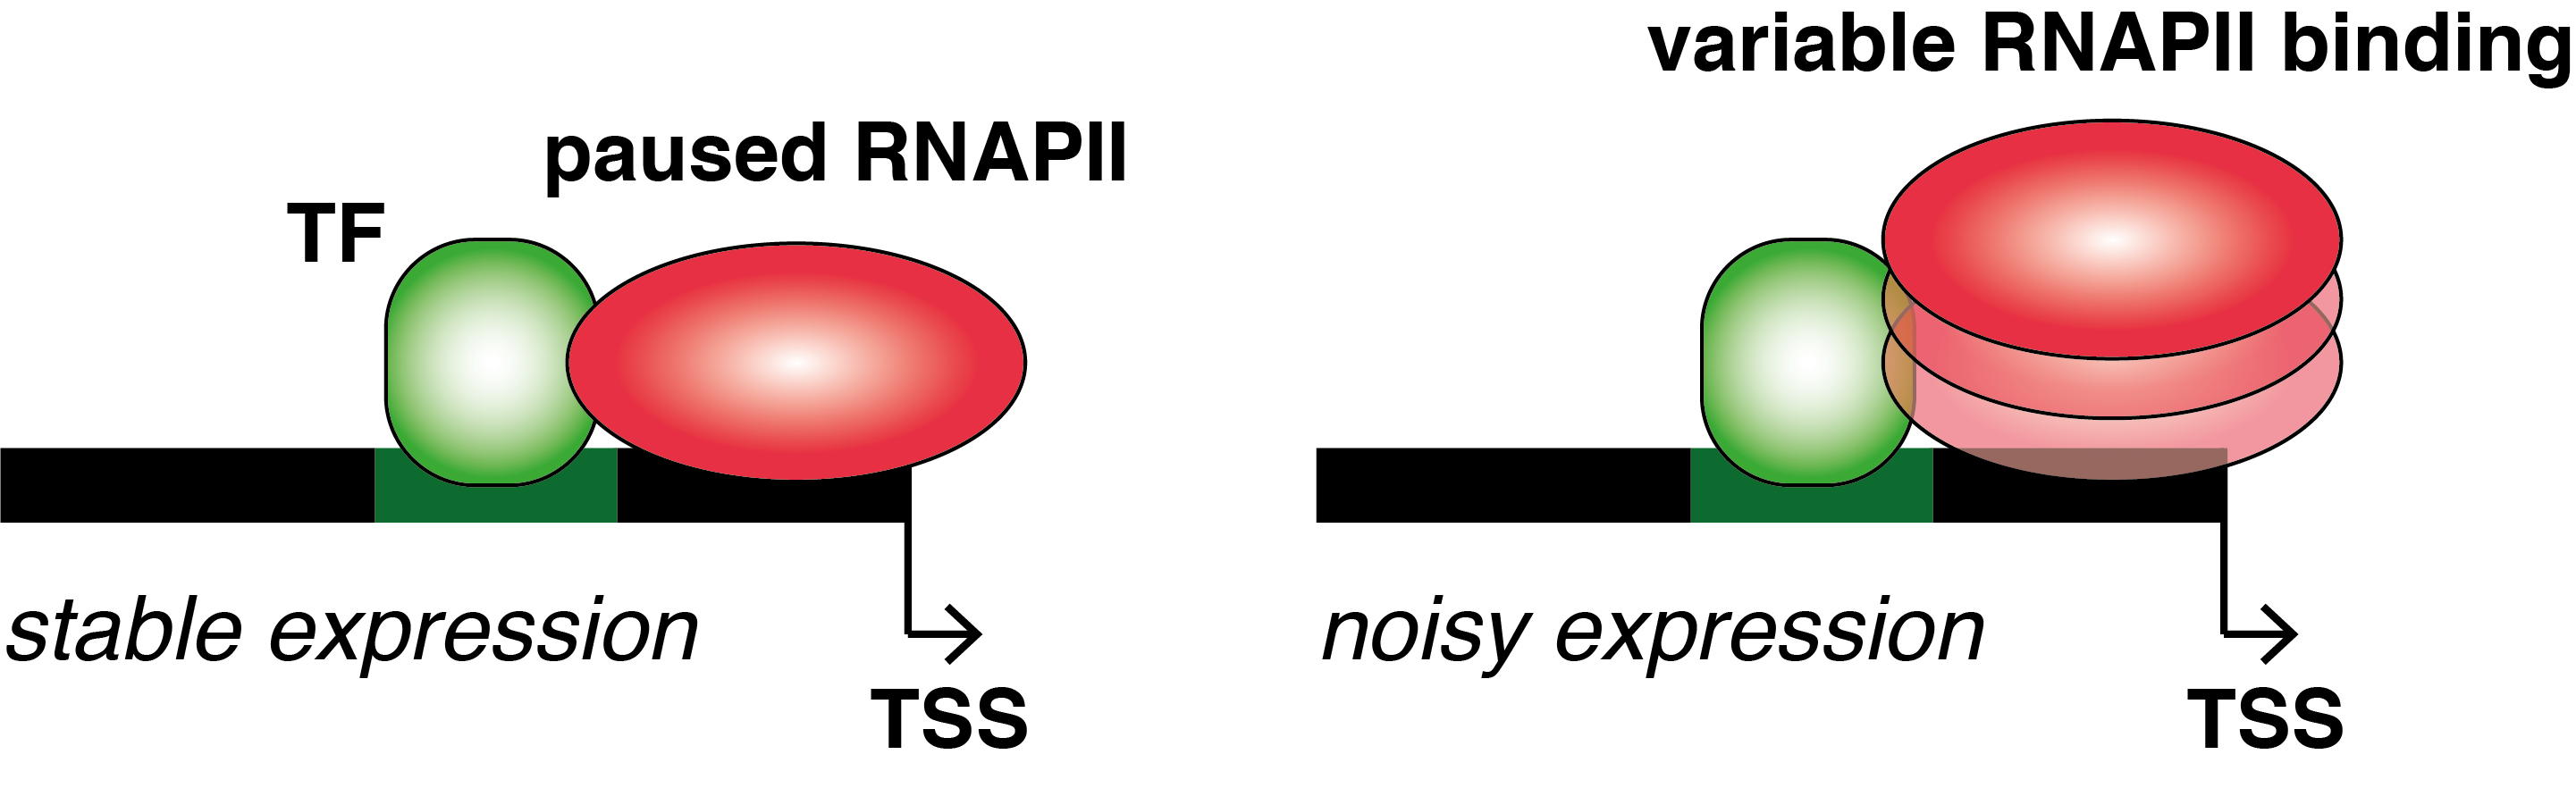
\includegraphics[width=\textwidth]{Fig_8.png}
\caption[Model comparison between the regression and non-regression BASiCS model]{\textbf{Model comparison between the regression and non-regression BASiCS model.}\\
(A)-(B) Results of differential testing between naive and activated CD4\plus{} T cells were compared between the regression and non-regression BASiCS models. As in section \ref{sec2:Tcell_activation}, genes with low mean expression ($\mu_i<50$) in both conditions were excluded from testing. \textbf{(A)} Overlap of differentially expressed genes (mean) using a minimum tolerance threshold $
\tau_0=2$ obtained using the regression and non-regression BASiCS models (EFDR = 10\%).\textbf{(B)} Upper panel: overlap of genes detected as non-differentially expressed using an stringent minimum tolerance threshold $\tau_0=0$ obtained using the regression and non-regression BASiCS models (EFDR = 10\%). Lower panel: overlap of differentially over-dispersed genes using a minimum tolerance threshold $\omega_0=\log_2(1.5)$ obtained using the regression and non-regression  BASiCS models for the 463 genes detected as non-differentially expressed by both models (EFDR = 10\%).\\}
\label{fig2:model_comparison}
\end{figure}

In this chapter, we exclude genes whose estimated mean expression parameter $\mu_i$ was below 1 from the differential testing. Furthermore, a $\log_2$ fold change threshold $\tau_0 = 1$ was adopted for mean expression testing. Unlike the more stringent threshold used in the first chapter ($\tau_0 = 2$), this choice allows us to detect more subtle changes in mean expression. Moreover, the default threshold $\psi_0 = 0.41$ was used for differential variability testing. The expected false discovery rate (EFDR) was controlled to 10\%. By using these thesholds, our model classifies genes into four categories based on their expression dynamics: down-regulated upon activation with (i) lower and (ii) higher variability, and up-regulated with (iii) lower and (iv) higher variability \textbf{(Fig.~\ref{fig2:immune_activation}A)}. \\

Genes with up-regulated expression upon activation and decreased expression variability encode components of the splicing machinery (e.g.~\textit{Sf3a3}, \textit{Plrg1}), RNA polymerase subunits (e.g.~\textit{Polr2l}, \textit{Polr1d}) as well as translation machinery components (e.g.~\textit{Ncl}, \textit{Naf1}) (see \textbf{Fig.~\ref{fig2:immune_activation}B}). These biosynthetic processes help naive T cells to rapidly enter a program of proliferation and effector molecule synthesis \citep{Tan2017,Araki2017}. Therefore, rapid, uniform up-regulation of these transcripts would assist such processes. This observation also confirms previous findings that the translational machinery is tightly regulated during early immune activation \citep{Martinez-jimenez2017}.\\ 

In contrast, genes with up-regulated expression and increased expression variability (see \textbf{Fig.~\ref{fig2:immune_activation}C}) include the death-inducing and inhibitory transmembrane ligands Fas ligand (\textit{Fasl}) and PD-L1 (\textit{Cd274}), the regulatory transcription factor Smad3 (\textit{Smad3}), and the TCR-induced transcription factor, Oct2 (\textit{Pou2f2}). Additionally, we detect a heterogeneous up-regulation in the mRNA expression of the autocrine/paracrine growth factor IL-2 (\textit{Il2}) upon immune activation. This is in line with previous reports of binary IL-2 expression within a population of activated T cells, which has been suggested to be necessary for a scalable antigen response \citep{Fuhrmann2016}. Heterogeneity in expression of these genes suggests that, despite their uniform up-regulation of biosynthetic machinery, the T cells in this early activation culture represent a mixed population with varying degrees of activation and/or regulatory potential. \\

\newpage

\begin{figure}[!h]
\centering
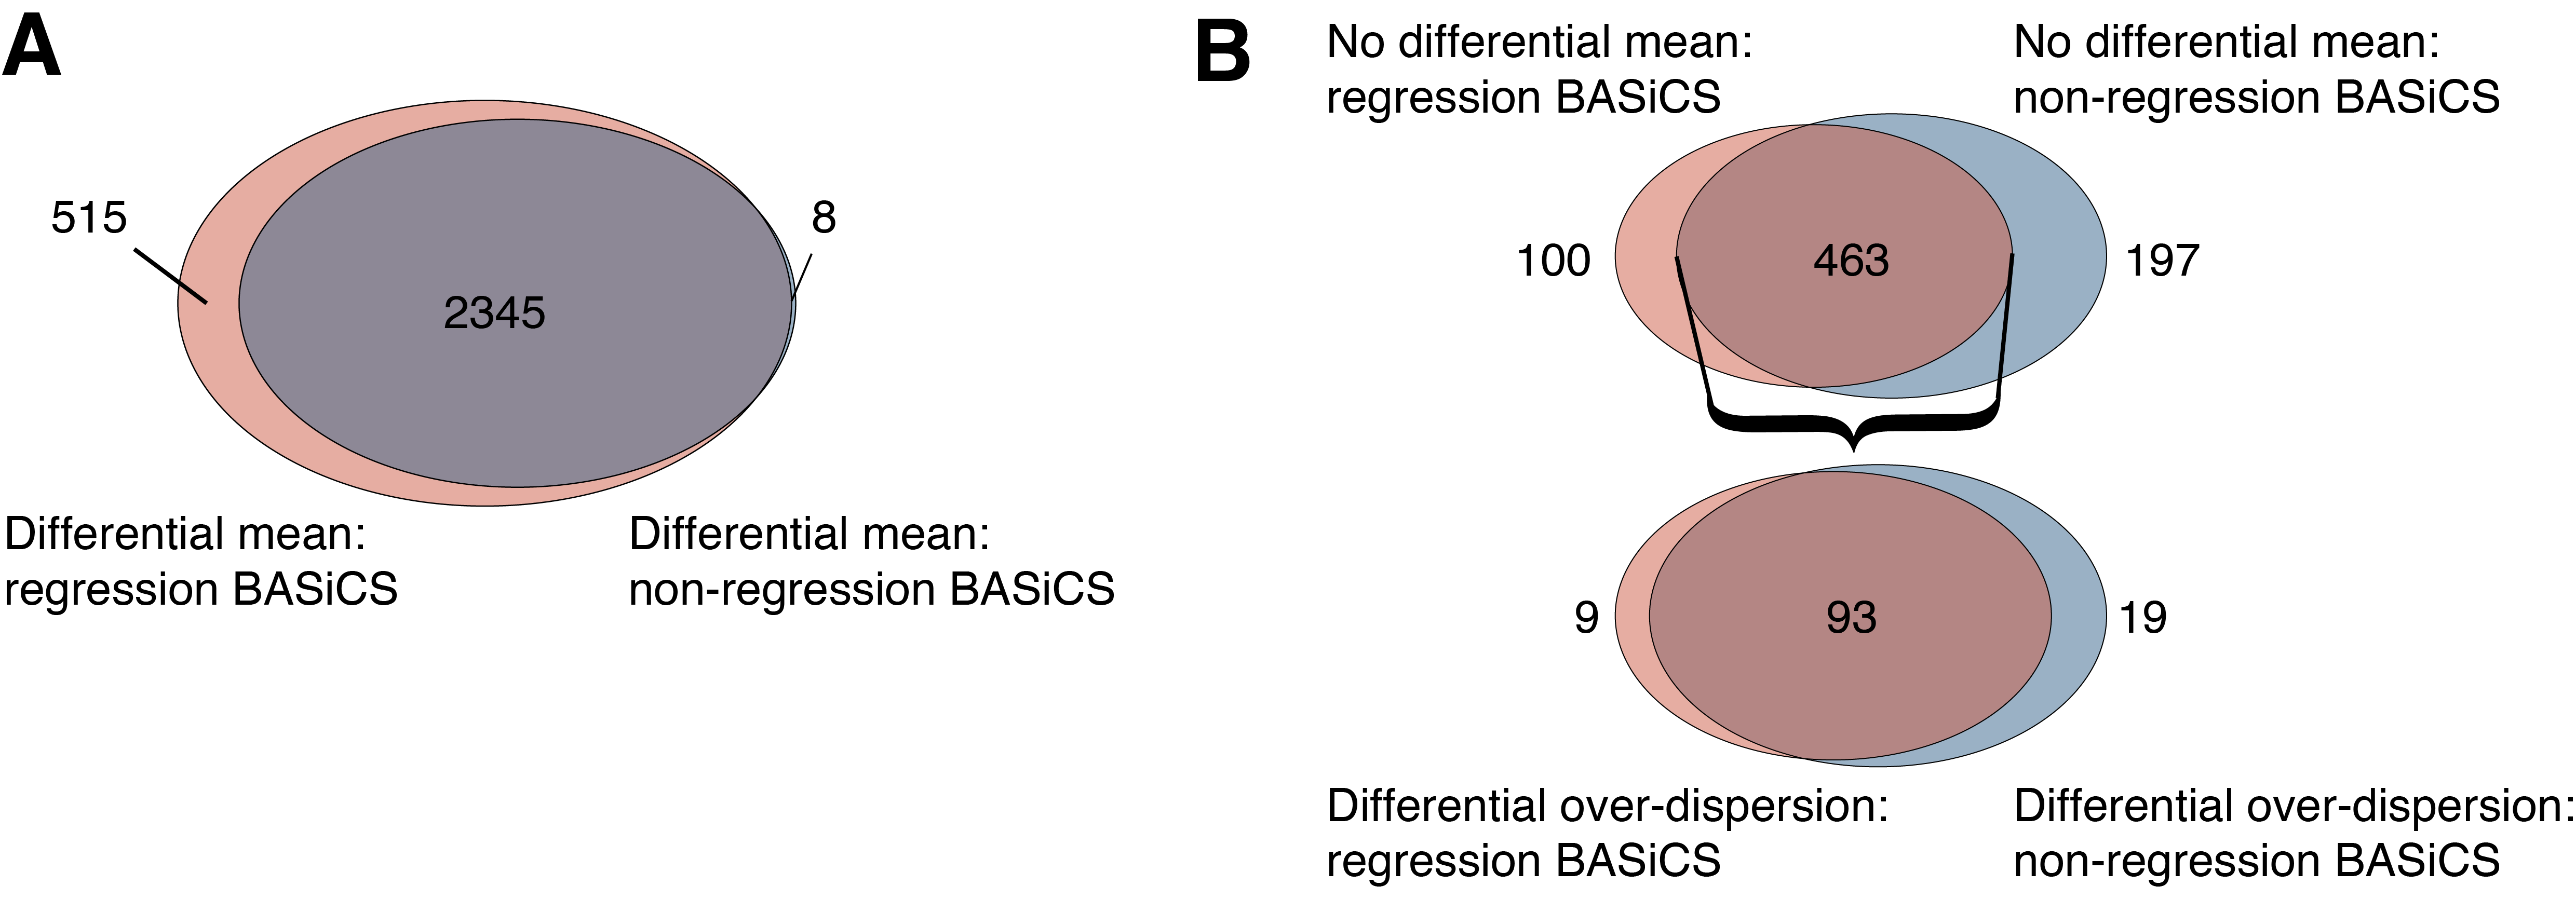
\includegraphics[width=0.75\textwidth]{Fig_9.png}
\caption[Changes in expression patterns during early immune activation]{\textbf{Changes in expression patterns during early immune activation in CD4\plus{} T cells.}\\
Differential testing (mean and residual over-dispersion) was performed between naive and activated murine CD4\plus{} T cells. This analysis uses a minimum tolerance threshold of $\tau_0=1$ for changes in mean expression and a minimum tolerance threshold of $\psi_0=0.41$ for differential residual over-dispersion testing (expected false discovery rate is fixed at 10\%). \textbf{(A)} For each gene, the difference in residual over-dispersion estimates (Active - Naive) is plotted versus the log$_2$ fold change in mean expression (Active/Naive). Genes with statistically significant changes in mean expression and variability are coloured based on their regulation (up/down-regulated, higher/lower variability).  \textbf{(B-C)} Denoised expression counts across the naive (purple) and active (green) CD4\plus{} T cell population are visualized for representative genes that (B) increase in mean expression and decrease in expression variability and (C) increase in mean expression as well as expression variability  upon immune activation. Each dot represents a single cell.}
\label{fig2:immune_activation}
\end{figure}

\newpage

For each of these gene sets, functional annotation analysis was performed using all tested genes as background. The functional annotation clustering tool in DAVID \citep{Dennis2003} was used to cluster annotation categories based on similarity and sort them according to their enrichment score. Here, we  list the top 3 functional annotation clusters per gene set and their corresponding enrichment score (ES):
\begin{itemize}
\item \textbf{Down-regulated with lower variability:} Pleckstrin homology domain (ES = 1.57), G protein signalling (ES = 1.51), glycosidase (ES = 1.49),
\item \textbf{Down-regulated with higher variability:} Ankyrin repeat-containing domain (ES = 2.19), GTPase mediated signalling (ES = 1.51), steroid biosynthesis (ES = 0.89), 
\item \textbf{Up-regulated with lower variability:} RNA polymerase (ES = 1.6), RNA binding (ES = 1.53), splicing (ES = 1.41),
\item \textbf{Up-regulated with higher variability:} Cytokine-cytokine receptor interaction (ES = 1.65), WD40 repeat (ES = 1.22), transcription (ES = 1.18).
\end{itemize}

We observe that for some genes (e.g.~\textit{Plrg1}), changes in variability are driven by a small number of outlier cells with high expression. The interpretation of these results is not trivial as it could reflect very subtle sub-structure or genuine changes in variability. To explore this, we performed the following synthetic experiment. We artificially created a mixed population of cells by combining 5 activated CD4\plus{} T cells with a population of 93 naive CD4\plus{} T cells. Subsequently, we performed a differential testing (mean and residual over-dispersion) between this mixed population and a \textit{pure} population of 93 naive CD4\plus{} T cells. As expected, this analysis shows an overall increase in variability in the mixed population. For example, among the genes that exhibit higher mean expression and higher residual over-dispersion in the mixed population, we found \textit{Il2} --- which is up-regulated upon CD4\plus{} T cell activation \textbf{(Fig.~\ref{fig2:mixture_population}A)}. Moreover, we observe that the genes in this category are enriched for those that are only expressed in the 5 activated CD4\plus{} T cells \textbf{(Fig.~\ref{fig2:mixture_population}B)}. This result suggests that differential variability testing can potentially uncover markers for heterogeneous cell states or cell types which can provide important biological insights. However, changes in residual over-dispersion that are driven by outliers can also reflect unwanted contamination 
(e.g.~mixed cell types), hence careful data filtering and clustering analysis should be performed prior to differential variability testing. 

\newpage

\begin{figure}[!h]
\centering
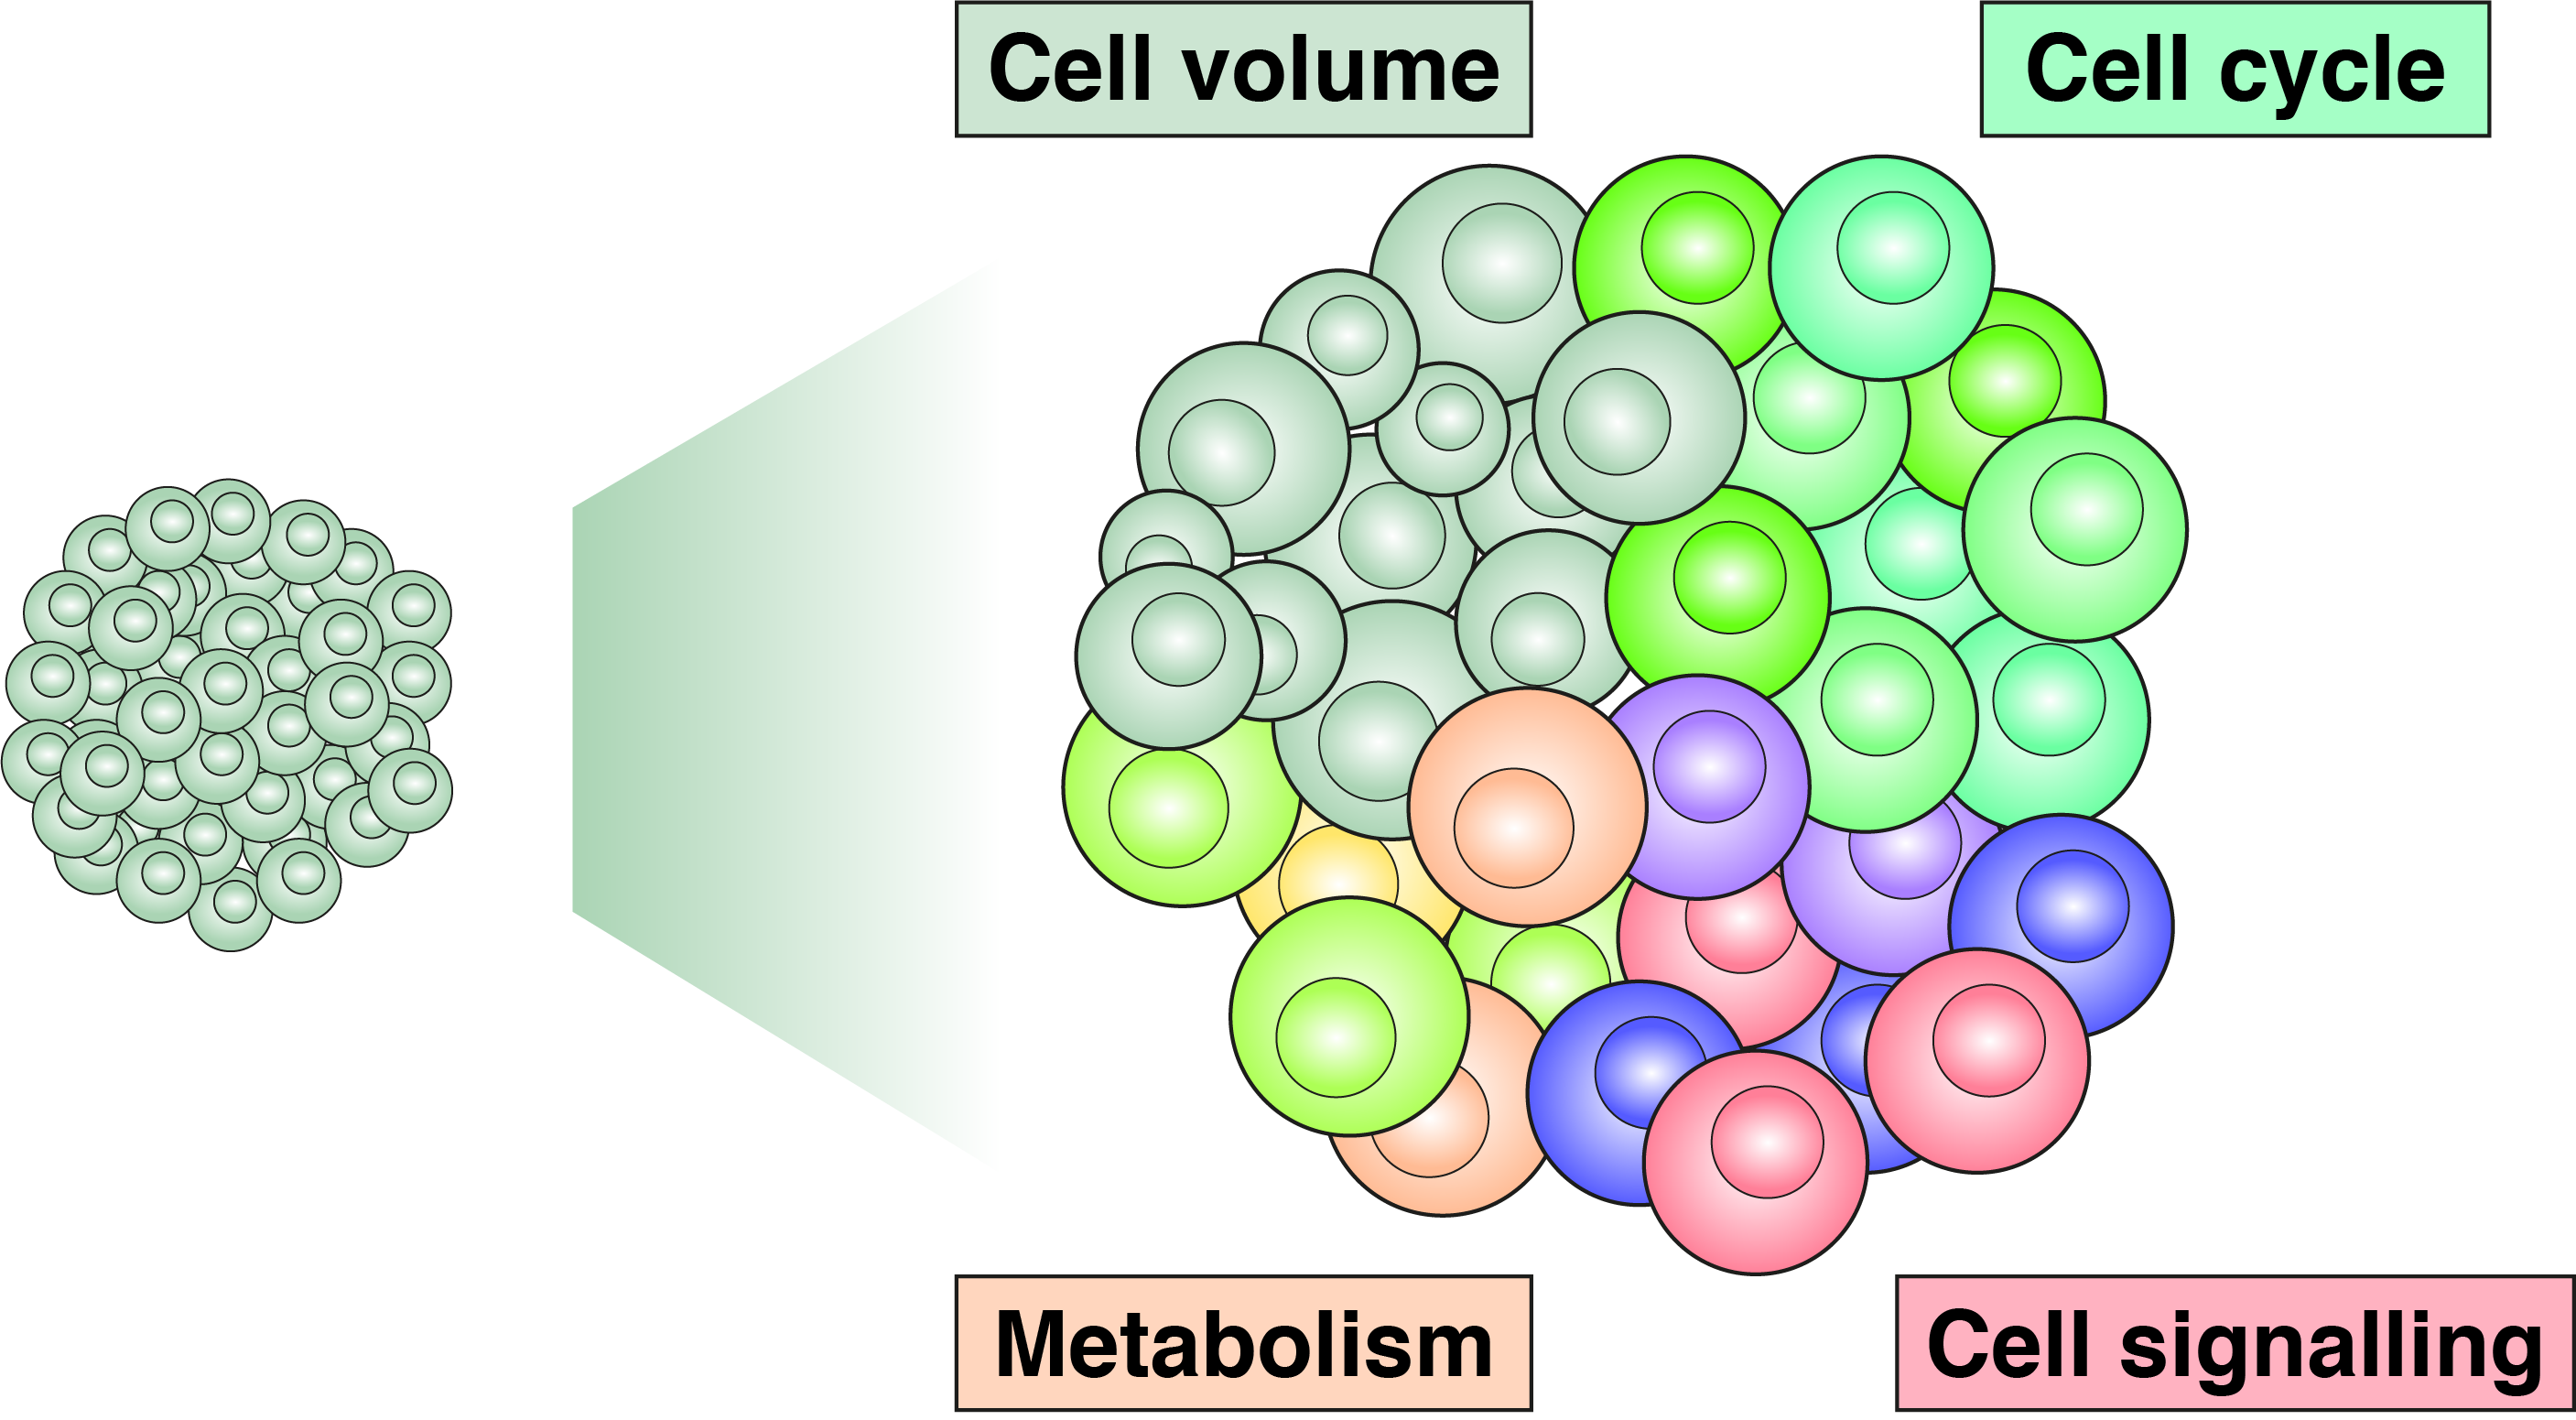
\includegraphics[width=\textwidth]{Fig_10.png}
\caption[Dissecting changes in variability driven by expression outliers]{\textbf{Dissecting changes in variability driven by expression outliers.}\\
5 activated CD4\plus{} T cells were combined with a population of 93 naive CD4\plus{} T cells. \textbf{(A)} Distribution of denoised expression counts for \textit{Il2} in a population of naive CD4\plus{} T cells (red) and the mixture population representing a mix of 93 naive and 5 activated CD4\plus{} T cells (blue). Each dot represents a single cell.\textbf{(B)} For the mixed population (93 naive and 5 activated CD4\plus{} T cells), heatmap of denoised expression counts for all genes highlighted to have increased mean expression and increased variability in the mixed population.}
\label{fig2:mixture_population}
\end{figure}


In summary, our approach allows us to extend the finding in section \ref{sec1:Tcell_activation}, dissecting immune-response genes into two functional sets: (i) homogeneous up-regulation of biosynthetic machinery components and (ii) heterogeneous up-regulation of several immunoregulatory genes.

\subsection{Expression dynamics during \textit{in vivo} CD4\plus{} T cell differentiation}

In contrast to the quick transcriptional switch that occurs within hours of naive T cell activation, transcriptional changes during cellular differentiation processes are more subtle and were found to be coupled with changes in variability prior to cell fate decisions \citep{Richard2016, Mojtahedi2016}. Here, we apply our method to study changes in expression variability during CD4\plus{} T cell differentiation after malaria infection using the dataset introduced by \cite{Lonnberg2017}. In particular, we focus on samples collected 2, 4 and 7 days post-malaria infection, for which more than 50 cells are available.\\

To study global changes in over-dispersion along the differentiation time course, we first compared posterior estimates for the gene-specific parameter $\delta_i$, focusing on the 126 genes for which mean expression does not change ($\tau_0 = 0$) \textbf{(Fig.~\ref{fig2:immune_differentiation}A)}. This analysis suggests that the expression of these genes is most tightly regulated at day 4, when cells are in a highly proliferative state. Moreover, between day 4 and day 7, the cell population becomes more heterogeneous. This is in line with the emergence of differentiated Th1 and Tfh cells that was observed by \cite{Lonnberg2017}. \\

\begin{figure}[!h]
\centering
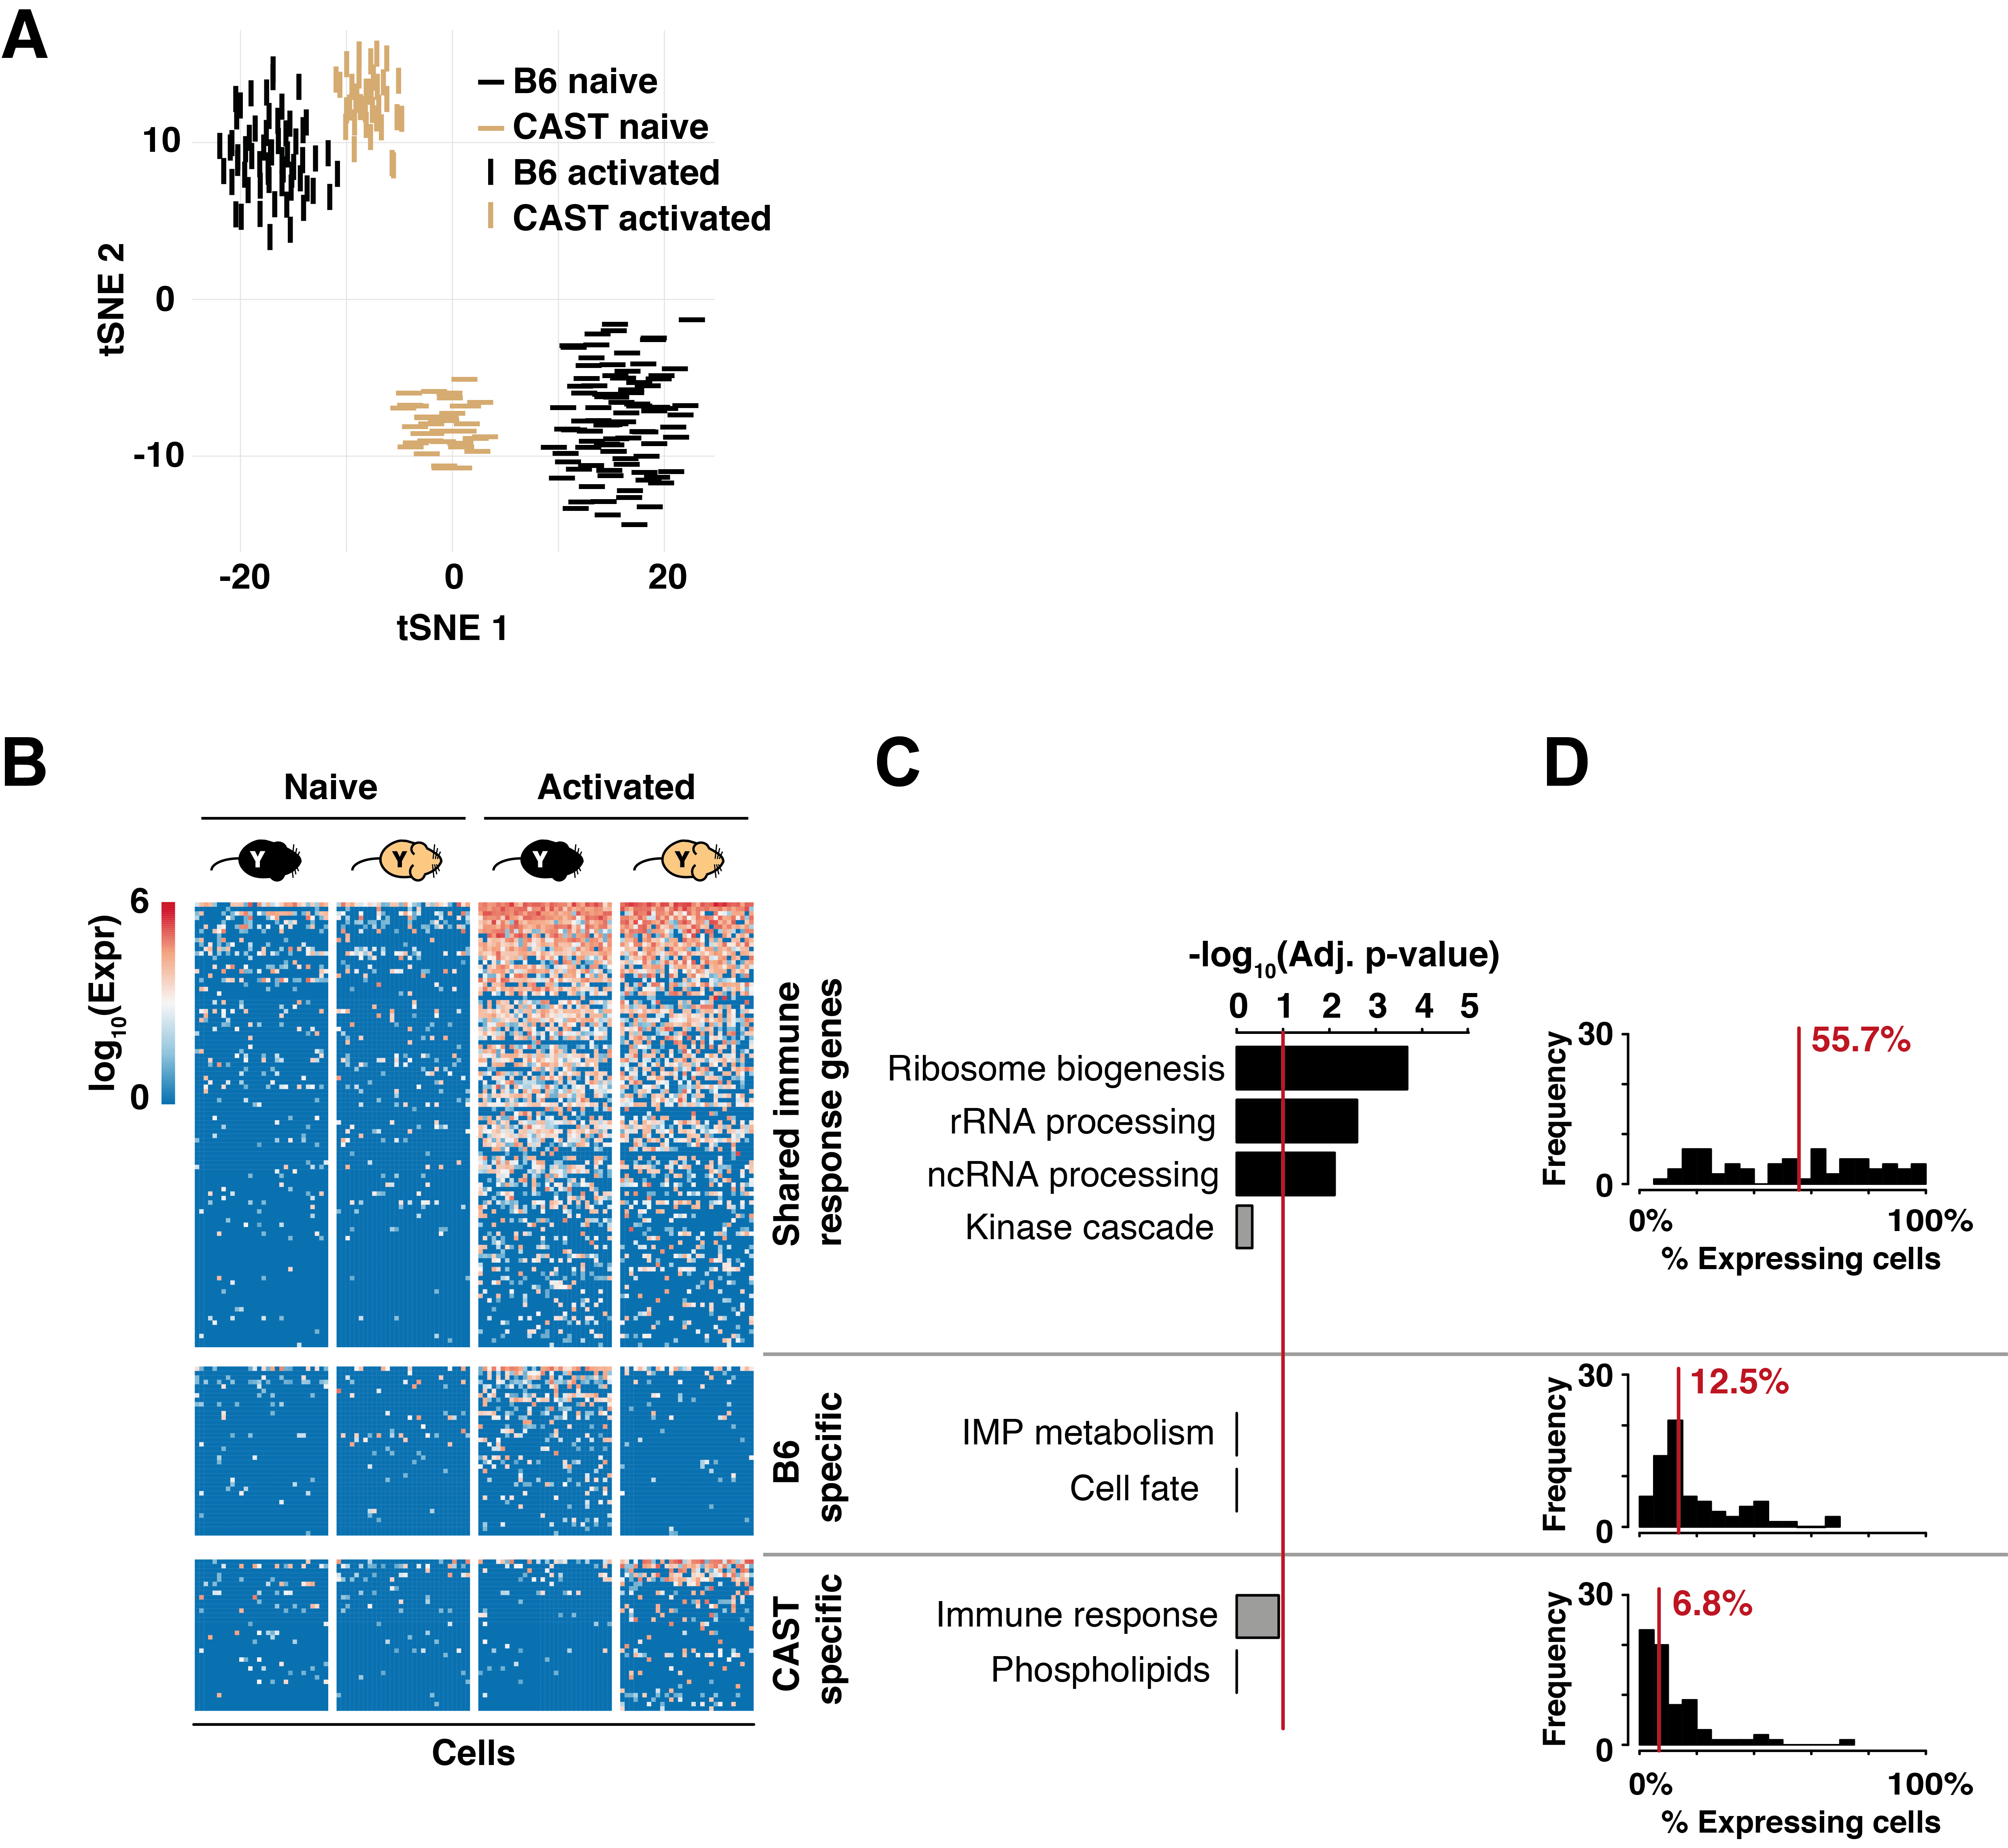
\includegraphics[width=\textwidth]{Fig_11.png}
\caption[Dynamics of expression variability throughout CD4\plus{} T cell differentiation]{\textbf{Dynamics of expression variability throughout CD4\plus{} T cell differentiation.}\\
Analysis was performed on CD4\plus{} T cells assayed 2 days, 4 days and 7 days after \textit{Plasmodium} infection. Changes in residual over-dispersion were tested using a minimum tolerance threshold of $\psi_0=0.41$ (expected false discovery rate is fixed at 10\%). \textbf{(A)} Distribution of posterior estimates of over-dispersion parameters $\delta_i$ for genes that exhibit no changes in mean expression across the differentiation time course. Changes in mean expression were tested using a minimum tolerance threshold of $\tau_0=0$ (expected false discovery rate is fixed at 10\%). \textbf{(B)} Posterior estimates for residual over-dispersion parameters  $\epsilon_i$, focusing on genes with statistically significant changes in expression variability between time points. Gene set size is indicated for each plot.\textbf{(C-D)} Denoised expression counts across cell populations at day 2 (yellow) and day 4 (red) post infection is visualized for representative genes that (C) increase or (D) decrease in variability during differentiation. Each dot represents a single cell.\\}
\label{fig2:immune_differentiation}
\end{figure}

We next exploited the residual over-dispersion parameters to identify changes in variability (irrespective of changes in mean expression) between consecutive time points. For this, we first removed all genes that are expressed in fewer than 2 cells in at least one time point. Separating these genes by whether their variability increases or decreases ($\psi_0 = 0.41$) between time points revealed four different patterns \textbf{(Fig.~\ref{fig2:immune_differentiation}B)}. These include genes whose variability systematically increases (or decreases) as well as patterns where variability is highest (or lowest) at day 4. \\

The differential variability analysis between day 2 and day 4, revealed  changes in expression variability for a set of immune-related genes \textbf{(Fig.~\ref{fig2:immune_differentiation}C-D)}. For example, expression of \textit{Cxcr5} which encodes the chemokine receptor that directs Tfh cells to the B cell follicles \citep{Crotty2014}, strongly increases in variability on day 4. This finding agrees with results from \cite{Lonnberg2017}, where Tfh and Th1 differentiation was observed to be transcriptionally detectable at day 4 within a subset of activated cells. A similar behaviour was observed for \textit{Tyk2} and \textit{Tigit}. The latter encodes a receptor that is expressed by a subset of Tfh cells and that was found to promote Tfh function \citep{Godefroy2015}. In contrast, we observe a decrease in variability between day 2 and day 4 for \textit{Ikzf4} (Treg-associated gene), \textit{Ly6c1} (expressed by effector T cells) and \textit{Tbx21} (encoding the Th1 lineage-defining transcription factor Tbet). \\

We next selected gene sets listed in \cite{Lonnberg2017} to visualize their changes in mean expression and residual over-dispersion. The first set of genes is taken from Figure 3E of the original publication, which filtered genes based on their association with the bifurcation of Th1 and Tfh differentiation. The second set of genes with sequential peak expression over pseudotime is taken from Figure 5A of the original publication, which were selected based on immunological relevance from a list of dynamic genes during \textit{in vivo} differentiation. For the genes that were detected to be lineage-associated, we detected a continuous increase in expression of Th1-associated genes but not Tfh-associated genes \textbf{(Fig.~\ref{fig2:immune_differentiation2}A)} with the majority of changes in variability for these genes occurring between day 2 and day 4. \\

Finally, we examined immune-related genes (\textit{Il2ra, Tbx21, Il2rb, Cxcr5, Selplg, Id2, Ifng, Icos, Ifngr1}) that were previously described as showing differences in their peak expression over the pseudo time-course of differentiation \citep{Lonnberg2017} \textbf{(Fig.~\ref{fig2:immune_differentiation2}B)}. From this list, the lineage-associated genes \textit{Tbx21} and \textit{Cxcr5} are up-regulated between days 2 and 4. However, these genes  exhibit opposite behaviours in terms of variability: \textit{Cxcr5} increases and \textit{Tbx21} decreases in variability between day 2 and day 4 \textbf{(Fig.~\ref{fig2:immune_differentiation2}C)}. The fact that variability of \textit{Tbx21} (Tbet) expression was highest on day 2 suggests that Tbet is up-regulated very early in differentiation, as seen in \cite{Lonnberg2017} and similar to \textit{in vitro} Th1 induction \citep{Szabo2000}. Moreover, this suggests that Th1 fate decisions (for at least a subset of cells) may be made even earlier than the differentiation bifurcation point identified on day 4 by the original study \citep{Lonnberg2017}. 

\newpage

\begin{figure}[!h]
  \begin{minipage}[c]{0.57\textwidth}
    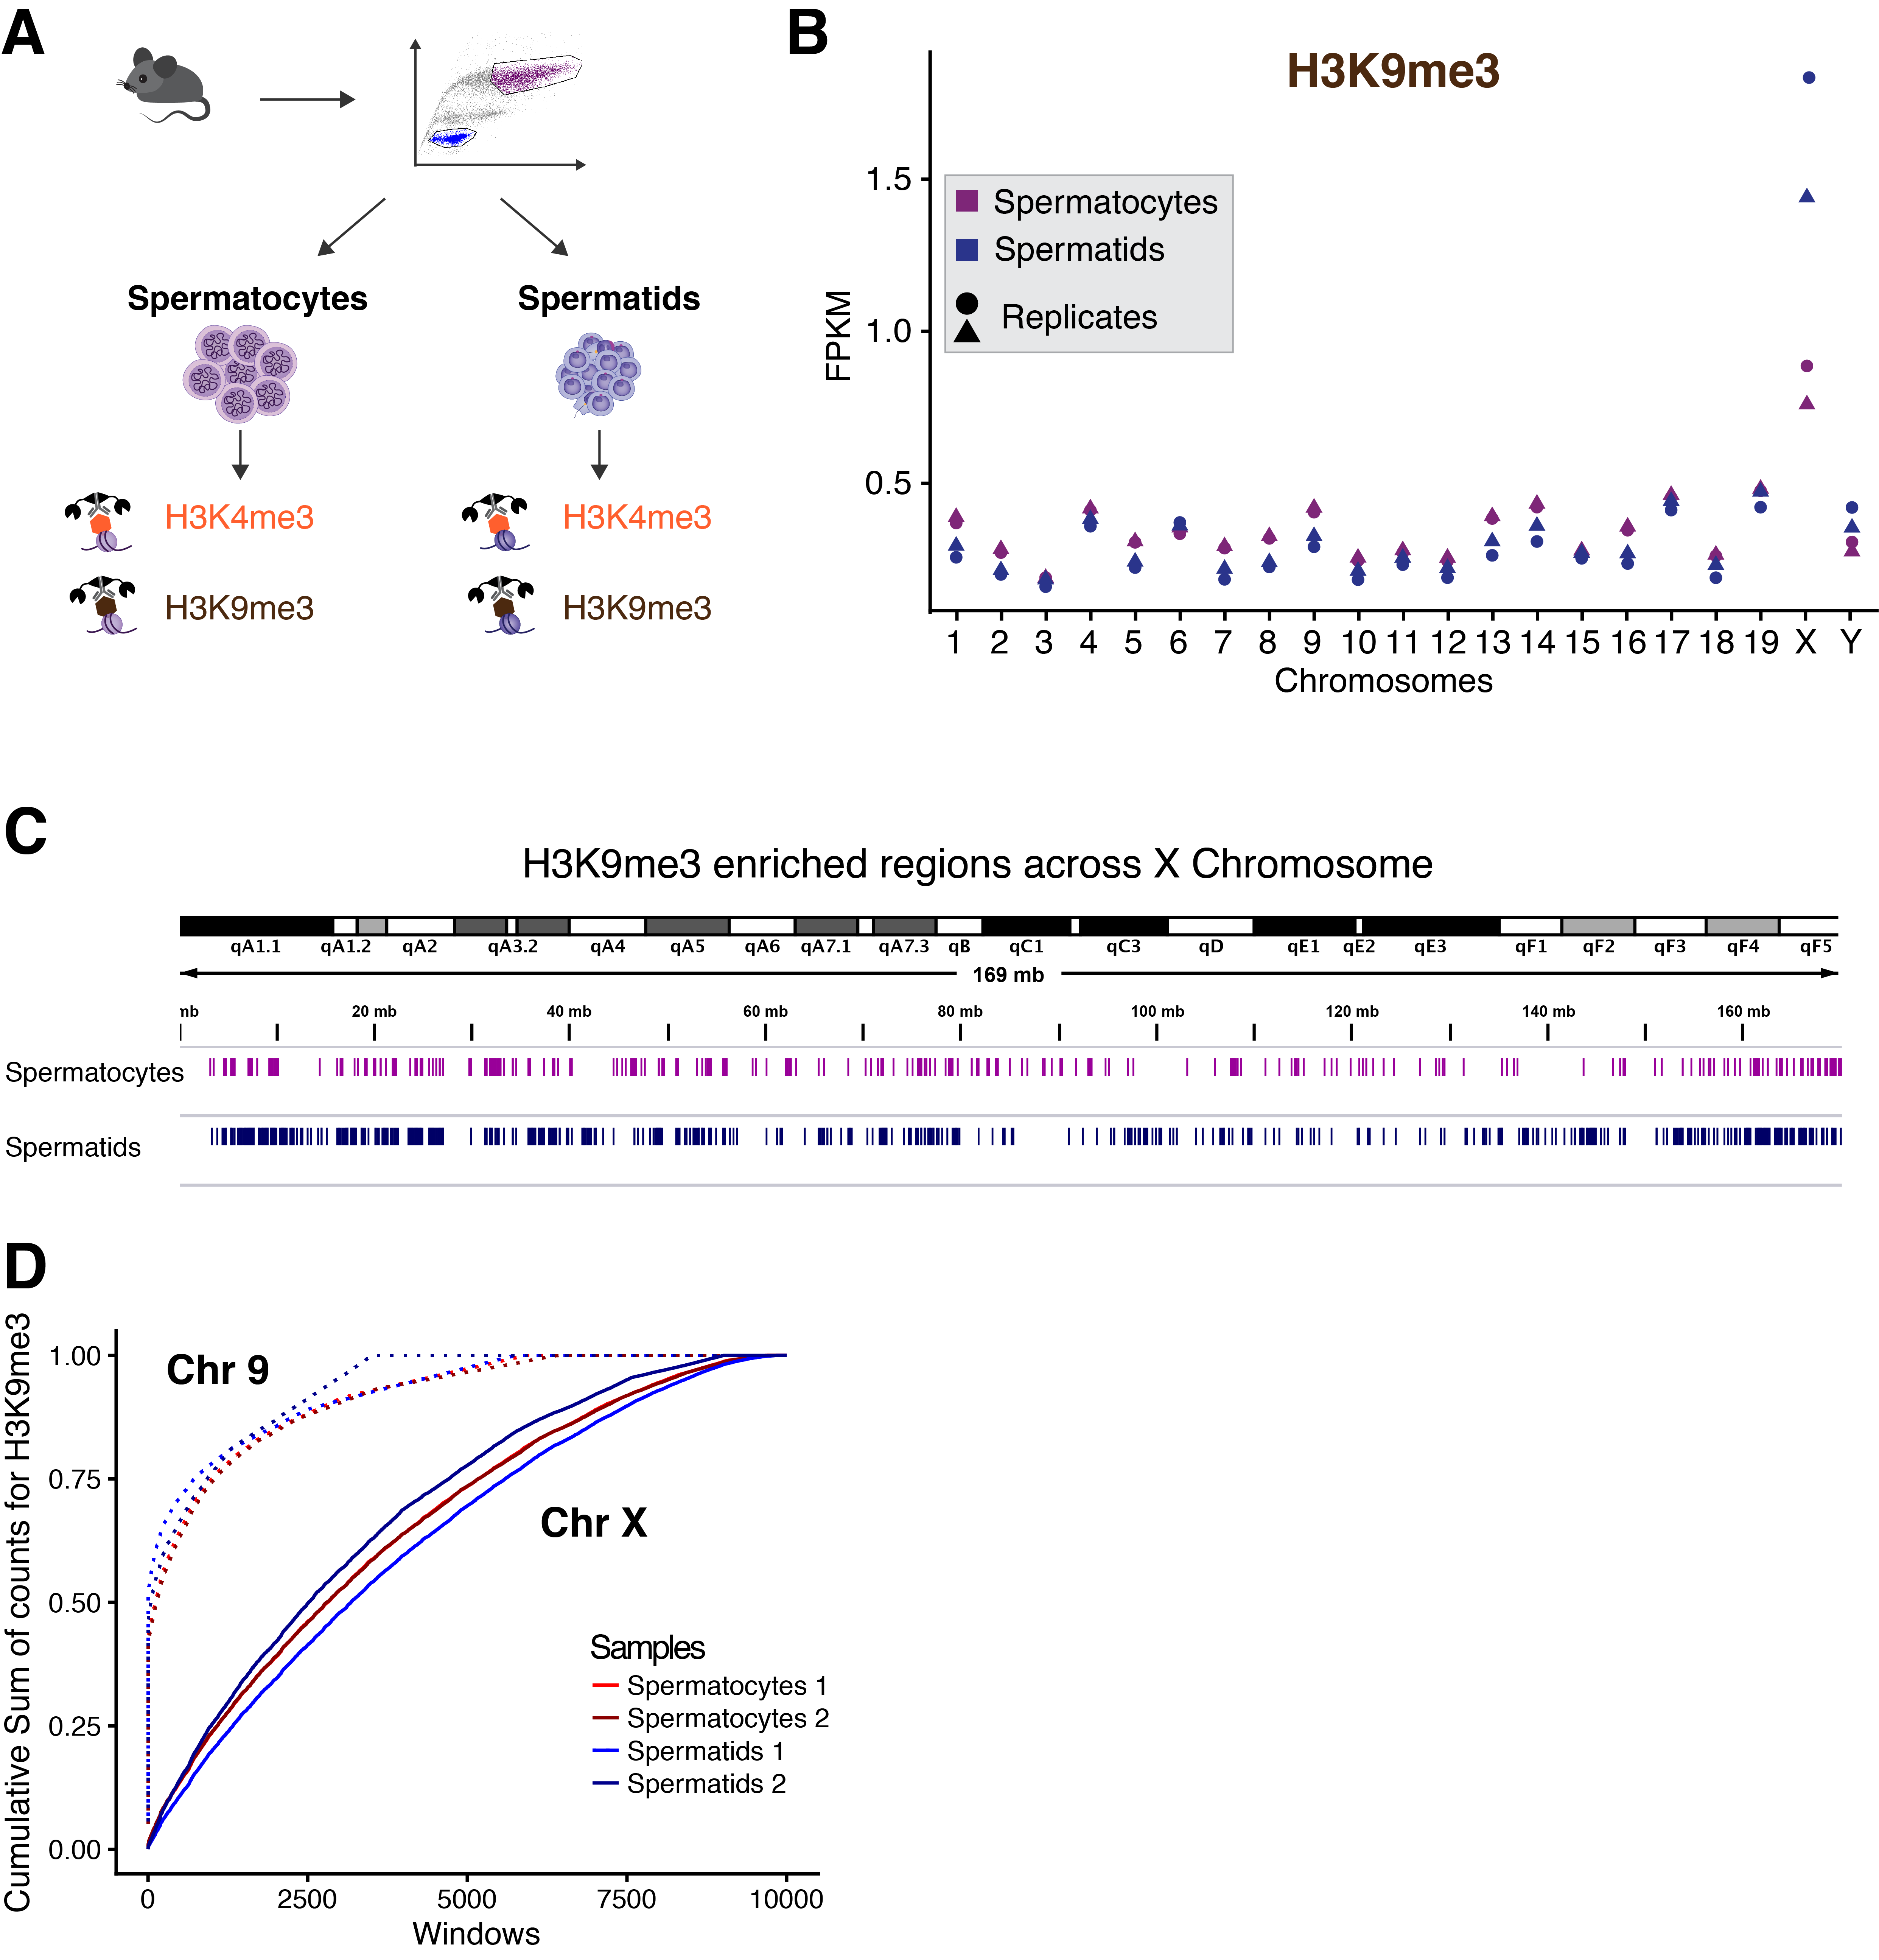
\includegraphics[width=\textwidth]{Fig_12.png}
  \end{minipage}\hfill
  \begin{minipage}[c]{0.4\textwidth}
\caption[Differential regulation of lineage-associated genes across differentiation]{\textbf{Differential regulation of Th1- and Tfh-associated genes across the differentiation process.}\\
Differential mean expression testing (minimum tolerance threshold $\tau_0=1$) and differential residual over-dispersion testing (minimum tolerance threshold $\psi_0=0.41$) was performed on cell populations between day 2 and day 4 as well as day 4 and day 7 controlling the EFDR to 10\%. Genes that increase in expression over time are marked with a red dot while genes that decrease in expression over time are marked with a blue dot. Similarly, genes that increase in variability over time are marked in purple while genes that decrease in variability over time are marked in green. Only genes that pass filtering are visualized. \textbf{(A)} Differential testing results are visualized for Th1- and Tfh-associated genes taken from Figure 3E in \cite{Lonnberg2017}. Genes are ordered based on their correlation with the Th1 trend assignment (top to bottom) or their correlation to Tfh trend assignment (bottom to top).\textbf{(B)} Differential testing results are visualized for important genes during CD4\plus{} T cell differentiation \citep[taken from Figure 5A in][]{Lonnberg2017}. Genes were ordered based on their peak expression point in pseudotime as defined by \cite{Lonnberg2017}. \textbf{(C)}\textit{Tbx21} (blue) and \textit{Cxcr5} (red) measured at day 2, day 4 and day 7 post-infection. Posterior estimates for residual over-dispersion parameters $\epsilon_i$ are plotted against posterior estimates for mean expression parameters $\mu_i$. Statistically significant changes in mean expression (DE, minimum tolerance threshold of $\tau_0=1$) and variability (DV, minimum tolerance threshold of $\psi_0=0.41$) are indicated for each comparison} \label{fig2:immune_differentiation2}
  \end{minipage}
\end{figure}

\newpage


\section{Discussion}

In recent years, the importance of modulating cell-to-cell transcriptional variation within cell populations for tissue function maintenance and development has become apparent \citep{BaharHalpern2015, Mojtahedi2016, Goolam2016}. Here, we present a statistical approach to robustly test changes in expression variability between cell populations using scRNA-Seq data. Our method uses a hierarchical Bayes formulation to extend the BASiCS framework by addressing (increasingly popular) experimental protocols where spike-in sequences are not available and by incorporating an additional set of residual over-dispersion parameters $\epsilon_i$ that are not confounded by changes in mean expression. Together, these extensions ensure a broader applicability of the BASiCS software and allow statistical testing of changes in variability that are not confounded by technical noise or mean expression.  \\ 

In general, stable gene-specific variability estimates ideally require a large and deeply sequenced dataset containing a homogeneous cell population \citep[the use of unique molecular identifiers for quantifying transcript counts can also improve variability estimation, see][]{Grun2014}. However, we observe that the regression BASiCS model leads to more stable inference that requires fewer cells to accurately estimate gene-specific summaries, particularly for lowly expressed genes. Despite this, careful considerations should be taken in extreme scenarios where the number of cells is small and/or the data is highly sparse (e.g.~droplet based approaches). These features of the data not only affect parameter estimation but also downstream differential testing. For sparse datasets with low numbers of cells, we recommend the use of a stringent minimum tolerance threshold and/or calibrating the test to a low expected false discovery rate (e.g.~1\%) to avoid detecting spurious signals. Moreover, if possible, an internal calibration can be performed to find a reasonable minimum tolerance threshold (e.g.~by randomly permuting cells between two groups to calibrate the null distribution of the differences between populations). \\

Our method allows characterisation of the extent and nature of variable gene expression in CD4\plus{} T cell activation and differentiation. Firstly, we observe that during acute activation of naive T cells, genes of the biosynthetic machinery are homogeneously up-regulated, while specific immune-related genes become more heterogeneously up-regulated. In particular, increased variability in expression of the apoptosis-inducing Fas ligand \citep{Strasser2009} and the inhibitory ligand PD-L1 \citep{Chikuma2016} suggests a mechanism by which newly activated cells might suppress re-activation of effector cells, thereby dynamically modulating the population response to activation. Likewise, more variable expression of Smad3, which translates inhibitory TGF$\beta$ signals into transcriptional changes \citep{Delisle2013}, may indicate increased diversity in cellular responses to this signal. Increased variability in \textit{Pou2f2} (Oct2) expression after activation suggests heterogeneous activities of the NF-$\kappa$B and/or NFAT signalling cascades that control its expression \citep{Mueller2013}.
Moreover, we detect up-regulated and more variable \textit{Il2} expression, suggesting heterogeneous IL-2 protein expression, which is known to enable T cell population responses \citep{Fuhrmann2016}. \\

Finally, we studied changes in gene expression variability during CD4\plus{} T cell differentiation towards a Th1 and Tfh cell state over a 7 day time course after \textit{in vivo} malaria infection \citep{Lonnberg2017}. Our analysis provides several insights into this differentiation system. Firstly, we observe a tighter regulation in gene expression among genes that do not change in mean expression during differentiation at day 4 at which divergence of Th1 and Tfh differentiation was previously identified \citep{Lonnberg2017}. This decrease in variability on day 4 is potentially due to induction of a strong pan-lineage proliferation program. However, we observe that not all genes follow this trend and uncover four different patterns of variability changes. Secondly, we observe that several Tfh and Th1 lineage-associated genes change in expression variability between days 2 and 4. For example, we noted a decrease in variability for one key Th1 regulator, \textit{Tbx21} (encoding Tbet), which suggests that a subset of cells may have already committed to the Th1 lineage at day 2. Three additional Th1 lineage-associated genes also followed this trend (\textit{Ahnak}, \textit{Ctsd}, \textit{Tmem154}). These data suggest that differentiation fate decisions may arise as early as day 2 in subpopulations within this system, resulting in high gene expression variability. Such an effect is in accordance with the early commitment to effector T cell fates that was previously observed during viral infection \citep{Choi2011}. As these results illustrate, diversity in differentiation state within a population of T cells can drive our differential variability results. To further disect these results, subsequent analyses such as the pseudotime inference used in \cite{Lonnberg2017} could be used to characterize a continuous differentiation process.\\

In sum, our model provides a robust tool for understanding the role of heterogeneity in gene expression during cell fate decisions. With the increasing use of scRNA-Seq to study this phenomenon, our and other related tools will become increasingly important.


